% **************************************************************************************************************
% A Classic Thesis Style
% An Homage to The Elements of Typographic Style
%
% Copyright (C) 2018 André Miede and Ivo Pletikosić
%
% If you like the style then I would appreciate a postcard. My address
% can be found in the file ClassicThesis.pdf. A collection of the
% postcards I received so far is available online at
% http://postcards.miede.de
%
% License:
% This program is free software; you can redistribute it and/or modify
% it under the terms of the GNU General Public License as published by
% the Free Software Foundation; either version 2 of the License, or
% (at your option) any later version.
%
% This program is distributed in the hope that it will be useful,
% but WITHOUT ANY WARRANTY; without even the implied warranty of
% MERCHANTABILITY or FITNESS FOR A PARTICULAR PURPOSE.  See the
% GNU General Public License for more details.
%
% You should have received a copy of the GNU General Public License
% along with this program; see the file COPYING.  If not, write to
% the Free Software Foundation, Inc., 59 Temple Place - Suite 330,
% Boston, MA 02111-1307, USA.
%
% PLEASE SEE ALSO THE AUTHORS' NOTE REGARDING THIS LICENSE
% IN THE DOCUMENTATION (ClassicThesis.pdf --> Chapter 1 / Chapter01.tex)
% ******************************************************************************
%%Customized for IIT Palakkad by Jasine Babu and Sravan Kumar Perumalla 
%% (jasine@iitpkd.ac.in, sravanperumalla@gmail.com) 
%% For reporting issues, IIT Palakkad users may contact jasine@iitpkd.ac.in  
%%******************************************************************************
\documentclass[ twoside,openright,titlepage,numbers=noenddot,%1headlines,
                headinclude,footinclude,cleardoublepage=empty,abstract=on,
                BCOR=5mm,paper=a4,fontsize=11pt
                ]{scrreprt}   

% ****************************************************************************************************
% classicthesis-config.tex
% formerly known as loadpackages.sty, classicthesis-ldpkg.sty, and classicthesis-preamble.sty
% Use it at the beginning of your ClassicThesis.tex, or as a LaTeX Preamble
% in your ClassicThesis.{tex,lyx} with % ****************************************************************************************************
% classicthesis-config.tex
% formerly known as loadpackages.sty, classicthesis-ldpkg.sty, and classicthesis-preamble.sty
% Use it at the beginning of your ClassicThesis.tex, or as a LaTeX Preamble
% in your ClassicThesis.{tex,lyx} with % ****************************************************************************************************
% classicthesis-config.tex
% formerly known as loadpackages.sty, classicthesis-ldpkg.sty, and classicthesis-preamble.sty
% Use it at the beginning of your ClassicThesis.tex, or as a LaTeX Preamble
% in your ClassicThesis.{tex,lyx} with \input{classicthesis-config}
% ****************************************************************************************************
% If you like the classicthesis, then I would appreciate a postcard.
% My address can be found in the file ClassicThesis.pdf. A collection
% of the postcards I received so far is available online at
% http://postcards.miede.de
% ****************************************************************************************************

\RequirePackage{silence} % :-\suppress an unnecessary warning in compilation
    \WarningFilter{scrreprt}{Usage of package `titlesec'}
    \WarningFilter{titlesec}{Non standard sectioning command detected}
    \WarningFilter{hyperref}{Token not allowed in a PDF string (PDFDocEncoding)}
   
% ****************************************************************************************************
% 0. Set the encoding of your files. UTF-8 is the only sensible encoding nowadays. If you can't read
% äöüßáéçèê∂åëæƒÏ€ then change the encoding setting in your editor, not the line below. If your editor
% does not support utf8 use another editor!
% ****************************************************************************************************
\PassOptionsToPackage{utf8}{inputenc}
  \usepackage{inputenc}

\PassOptionsToPackage{T1}{fontenc} % T2A for cyrillics
  \usepackage{fontenc}

\PassOptionsToPackage{final}{microtype}  %jasine
\usepackage[final]{microtype} %jasine

\emergencystretch=1em

% *******************************************************************************************************************
% Note : Do not edit above this line
% Note : Do not edit options to classicthesis given below except the options drafting, printready and numsupervisors
% and eulermath
% 
% *******************************************************************************************************************
\PassOptionsToPackage{
   tocaligned=false, 
  dottedtoc=true,
  eulerchapternumbers=true, 
  linedheaders=false,      
  eulermath=true, %true, %false %recommended value is true. If false is used, cmmodern will be used.
  beramono=true,   
  palatino=true,    
  style=classicthesis, 
  floatperchapter=true,     % numbering per chapter for all floats (i.e., Figure 1.1)
  numsupervisors=one, %one %two %three %set according to your number of supervisors
  %drafting=true,    % print version information on the bottom of the pages only for draft
  drafting=false, % for final version this line is to be used
  printready=false %Enable this for making title page and hyperreflinks in colour for screen reading
  %printready=true  %Enable this for making title page and hyperreflinks in black for printing
 }{classicthesis}


% ****************************************************************************************************
% 2. Personal data and user ad-hoc commands (insert your own data here)
% ****************************************************************************************************

\newcommand{\myTitle}{Main Title of Your Thesis\xspace}
\newcommand{\mySubtitle}{Subtitle of Your Thesis\xspace}
\newcommand{\myDegree}{Doctor of Philosophy\xspace}
%\newcommand{\myDegree}{Master of Science \xspace}
%\newcommand{\myDegree}{Master of Science in Engineering \xspace}
\newcommand{\myName}{Your Full Name\xspace}
\newcommand{\myGender}{her\xspace}
%\newcommand{\myGender}{him\xspace}
\newcommand{\mySupervisorOne}{First Supervisor Name}
\newcommand{\mySupervisorTwo}{Second Supervisor Name}%used only if necessary
\newcommand{\mySupervisorThree}{Third Supervisor Name}%used only if necessary
\newcommand{\myDepartment}{Department of Computer Science and Engineering\xspace}
\newcommand{\myUni}{Indian Institute of Technology Palakkad\xspace}
\newcommand{\myLocation}{Palakkad\xspace}
\newcommand{\myTime}{Month YYYY\xspace}
\newcommand{\myVersion}{\classicthesis}
% ********************************************************************
% Setup, finetuning, and useful commands
% ********************************************************************
\providecommand{\mLyX}{L\kern-.1667em\lower.25em\hbox{Y}\kern-.125emX\@}
\newcommand{\ie}{i.\,e.}
\newcommand{\Ie}{I.\,e.}
\newcommand{\eg}{e.\,g.}
\newcommand{\Eg}{E.\,g.}
% ****************************************************************************************************


% ****************************************************************************************************
% 3. Loading some handy packages
% ****************************************************************************************************
% ********************************************************************
% Packages with options that might require adjustments
% ********************************************************************
\PassOptionsToPackage{ngerman,american}{babel} % change this to your language(s), main language last
\usepackage{babel}

\usepackage{csquotes}
%%%%%You may change the reference format to any of the options given agaist the parameters. 
%%%%%It is suggested that you maintain compatibility with natbib.
\PassOptionsToPackage{%
  %backend=biber,bibencoding=utf8, %instead of bibtex
  backend=bibtex8,bibencoding=ascii,%
  language=auto,%
  style=numeric-comp,%
  %style=authoryear-comp, % Author 1999, 2010
  %bibstyle=authoryear,dashed=false, % dashed: substitute rep. author with ---
  sorting=nyt, % name, year, title
  maxbibnames=10, % default: 3, et al.
  %backref=true,%
  natbib=true % natbib compatibility mode (\citep and \citet still work)
}{biblatex}
\usepackage{biblatex}

\PassOptionsToPackage{fleqn}{amsmath}       % math environments and more by the AMS
   \usepackage{amsmath}

\usepackage{amssymb}
\usepackage{wasysym}
\usepackage{amsthm} 
\usepackage{mathrsfs}
\usepackage{mathtools}
\usepackage{epsfig}
%%%%Theorem like environments follow chapterwise numbering, 
%%%%only exceptions being 'Remark' and 'Note'.
%%%%Do not edit this basic setting, if you are adding more such environments.
\theoremstyle{plain}% default
\newtheorem{theorem}{Theorem}[section]
\newtheorem{lemma}[theorem]{Lemma}
\newtheorem{proposition}[theorem]{Proposition}
\newtheorem{corollary}[theorem]{Corollary}
\newtheorem{property}[theorem]{Property}

\theoremstyle{definition}
\newtheorem{definition}[theorem]{Definition}
\newtheorem{conjecture}[theorem]{Conjecture}
\newtheorem{example}[theorem]{Example}
\newtheorem{observation}[theorem]{Observation}

\theoremstyle{remark}
\newtheorem*{remark}{Remark}
\newtheorem*{note}{Note}
\newtheorem{claim}{Claim}[chapter]

\usepackage[ruled,vlined,algochapter]{algorithm2e}

% ********************************************************************
% General useful packages
% ********************************************************************
\usepackage{graphicx} %
\usepackage{scrhack} % fix warnings when using KOMA with listings package
\usepackage{xspace} % to get the spacing after macros right
\PassOptionsToPackage{printonlyused,smaller}{acronym}
  \usepackage{acronym} % nice macros for handling all acronyms in the thesis
  \def\bflabel#1{{\acsfont{#1}\hfill}}
  \def\aclabelfont#1{\acsfont{#1}}
% ****************************************************************************************************
%\usepackage{pgfplots} % External TikZ/PGF support (thanks to Andreas Nautsch)
%\usetikzlibrary{external}
%\tikzexternalize[mode=list and make, prefix=ext-tikz/]
% ****************************************************************************************************




% ****************************************************************************************************
% 4. Setup floats: tables, (sub)figures, and captions
%%%Do not edit this setting
% ****************************************************************************************************
\usepackage{tabularx} % better tables
  \setlength{\extrarowheight}{3pt} % increase table row height
\newcommand{\tableheadline}[1]{\multicolumn{1}{l}{\spacedlowsmallcaps{#1}}}
\newcommand{\myfloatalign}{\centering} % to be used with each float for alignment
\usepackage{subfig}
% ****************************************************************************************************


% ****************************************************************************************************
% 5. Setup code listings
%%Do not edit this setting
% ****************************************************************************************************
\usepackage{listings}
%\lstset{emph={trueIndex,root},emphstyle=\color{BlueViolet}}%\underbar} % for special keywords
\lstset{language=[LaTeX]Tex,%C++,
  morekeywords={PassOptionsToPackage,selectlanguage},
  keywordstyle=\color{CTkeyword},%\bfseries,
  basicstyle=\small\ttfamily,
  %identifierstyle=\color{NavyBlue},
  commentstyle=\color{CTcomment}\ttfamily,
  stringstyle=\rmfamily,
  numbers=none,%left,%
  numberstyle=\scriptsize,%\tiny
  stepnumber=5,
  numbersep=8pt,
  showstringspaces=false,
  breaklines=true,
  %frameround=ftff,
  %frame=single,
  belowcaptionskip=.75\baselineskip
  %frame=L
}
% ****************************************************************************************************

%%%%Note that for list of symbols to be inluded the following commands needs to be executed
%%%%pdflatex ClassicThesis.tex
%%%%makeindex ClassicThesis.nlo -s nomencl.ist -o ClassicThesis.nls
%%%%pdflatex ClassicThesis.tex
\usepackage{nomencl}
\makenomenclature
\renewcommand{\nomname}{List of Symbols}
% ****************************************************************************************************
% 6. Last calls before the bar closes
% ****************************************************************************************************
% ********************************************************************
% Her Majesty herself
% ********************************************************************
\usepackage{classicthesis}


% ********************************************************************
% Fine-tune hyperreferences (hyperref should be called last)
%%%Do not edit this setting
% ********************************************************************
\hypersetup{%
  colorlinks=true, linktocpage=true, pdfstartpage=3, pdfstartview=FitV,%
  breaklinks=true, pageanchor=true,%
  pdfpagemode=UseNone, %
  plainpages=false, bookmarksnumbered, bookmarksopen=true, bookmarksopenlevel=1,%
  hypertexnames=true, pdfhighlight=/O,%
  urlcolor=CTurl, linkcolor=CTlink, citecolor=CTcitation, %
  pdftitle={\myTitle},%
  pdfauthor={\textcopyright\ \myName, \myUni},%
  pdfsubject={},%
  pdfkeywords={},%
  pdfcreator={pdfLaTeX},%
  pdfproducer={LaTeX with hyperref and classicthesis}%
}

%%%%%%%%%Do not edit below this line %%%%%%%%%%%%%%%%%%%%%%%%%%%%%%%%%

% ********************************************************************
% Setup autoreferences (hyperref and babel)
% ********************************************************************
% There are some issues regarding autorefnames
% http://www.tex.ac.uk/cgi-bin/texfaq2html?label=latexwords
% you have to redefine the macros for the
% language you use, e.g., american, ngerman
% (as chosen when loading babel/AtBeginDocument)
% ********************************************************************
\makeatletter
\@ifpackageloaded{babel}%
  {%
    \addto\extrasamerican{%
      \renewcommand*{\figureautorefname}{Figure}%
      \renewcommand*{\tableautorefname}{Table}%
      \renewcommand*{\partautorefname}{Part}%
      \renewcommand*{\chapterautorefname}{Chapter}%
      \renewcommand*{\sectionautorefname}{Section}%
      \renewcommand*{\subsectionautorefname}{Section}%
      \renewcommand*{\subsubsectionautorefname}{Section}%
    }%
    \addto\extrasngerman{%
      \renewcommand*{\paragraphautorefname}{Absatz}%
      \renewcommand*{\subparagraphautorefname}{Unterabsatz}%
      \renewcommand*{\footnoteautorefname}{Fu\"snote}%
      \renewcommand*{\FancyVerbLineautorefname}{Zeile}%
      \renewcommand*{\theoremautorefname}{Theorem}%
      \renewcommand*{\appendixautorefname}{Anhang}%
      \renewcommand*{\equationautorefname}{Gleichung}%
      \renewcommand*{\itemautorefname}{Punkt}%
    }%
      % Fix to getting autorefs for subfigures right (thanks to Belinda Vogt for changing the definition)
      \providecommand{\subfigureautorefname}{\figureautorefname}%
    }{\relax}
\makeatother

\listfiles
\linespread{1.1} % a bit more for Palatino
% ****************************************************************************************************
% If you like the classicthesis, then I would appreciate a postcard.
% My address can be found in the file ClassicThesis.pdf. A collection
% of the postcards I received so far is available online at
% http://postcards.miede.de
% ****************************************************************************************************

\RequirePackage{silence} % :-\suppress an unnecessary warning in compilation
    \WarningFilter{scrreprt}{Usage of package `titlesec'}
    \WarningFilter{titlesec}{Non standard sectioning command detected}
    \WarningFilter{hyperref}{Token not allowed in a PDF string (PDFDocEncoding)}
   
% ****************************************************************************************************
% 0. Set the encoding of your files. UTF-8 is the only sensible encoding nowadays. If you can't read
% äöüßáéçèê∂åëæƒÏ€ then change the encoding setting in your editor, not the line below. If your editor
% does not support utf8 use another editor!
% ****************************************************************************************************
\PassOptionsToPackage{utf8}{inputenc}
  \usepackage{inputenc}

\PassOptionsToPackage{T1}{fontenc} % T2A for cyrillics
  \usepackage{fontenc}

\PassOptionsToPackage{final}{microtype}  %jasine
\usepackage[final]{microtype} %jasine

\emergencystretch=1em

% *******************************************************************************************************************
% Note : Do not edit above this line
% Note : Do not edit options to classicthesis given below except the options drafting, printready and numsupervisors
% and eulermath
% 
% *******************************************************************************************************************
\PassOptionsToPackage{
   tocaligned=false, 
  dottedtoc=true,
  eulerchapternumbers=true, 
  linedheaders=false,      
  eulermath=true, %true, %false %recommended value is true. If false is used, cmmodern will be used.
  beramono=true,   
  palatino=true,    
  style=classicthesis, 
  floatperchapter=true,     % numbering per chapter for all floats (i.e., Figure 1.1)
  numsupervisors=one, %one %two %three %set according to your number of supervisors
  %drafting=true,    % print version information on the bottom of the pages only for draft
  drafting=false, % for final version this line is to be used
  printready=false %Enable this for making title page and hyperreflinks in colour for screen reading
  %printready=true  %Enable this for making title page and hyperreflinks in black for printing
 }{classicthesis}


% ****************************************************************************************************
% 2. Personal data and user ad-hoc commands (insert your own data here)
% ****************************************************************************************************

\newcommand{\myTitle}{Main Title of Your Thesis\xspace}
\newcommand{\mySubtitle}{Subtitle of Your Thesis\xspace}
\newcommand{\myDegree}{Doctor of Philosophy\xspace}
%\newcommand{\myDegree}{Master of Science \xspace}
%\newcommand{\myDegree}{Master of Science in Engineering \xspace}
\newcommand{\myName}{Your Full Name\xspace}
\newcommand{\myGender}{her\xspace}
%\newcommand{\myGender}{him\xspace}
\newcommand{\mySupervisorOne}{First Supervisor Name}
\newcommand{\mySupervisorTwo}{Second Supervisor Name}%used only if necessary
\newcommand{\mySupervisorThree}{Third Supervisor Name}%used only if necessary
\newcommand{\myDepartment}{Department of Computer Science and Engineering\xspace}
\newcommand{\myUni}{Indian Institute of Technology Palakkad\xspace}
\newcommand{\myLocation}{Palakkad\xspace}
\newcommand{\myTime}{Month YYYY\xspace}
\newcommand{\myVersion}{\classicthesis}
% ********************************************************************
% Setup, finetuning, and useful commands
% ********************************************************************
\providecommand{\mLyX}{L\kern-.1667em\lower.25em\hbox{Y}\kern-.125emX\@}
\newcommand{\ie}{i.\,e.}
\newcommand{\Ie}{I.\,e.}
\newcommand{\eg}{e.\,g.}
\newcommand{\Eg}{E.\,g.}
% ****************************************************************************************************


% ****************************************************************************************************
% 3. Loading some handy packages
% ****************************************************************************************************
% ********************************************************************
% Packages with options that might require adjustments
% ********************************************************************
\PassOptionsToPackage{ngerman,american}{babel} % change this to your language(s), main language last
\usepackage{babel}

\usepackage{csquotes}
%%%%%You may change the reference format to any of the options given agaist the parameters. 
%%%%%It is suggested that you maintain compatibility with natbib.
\PassOptionsToPackage{%
  %backend=biber,bibencoding=utf8, %instead of bibtex
  backend=bibtex8,bibencoding=ascii,%
  language=auto,%
  style=numeric-comp,%
  %style=authoryear-comp, % Author 1999, 2010
  %bibstyle=authoryear,dashed=false, % dashed: substitute rep. author with ---
  sorting=nyt, % name, year, title
  maxbibnames=10, % default: 3, et al.
  %backref=true,%
  natbib=true % natbib compatibility mode (\citep and \citet still work)
}{biblatex}
\usepackage{biblatex}

\PassOptionsToPackage{fleqn}{amsmath}       % math environments and more by the AMS
   \usepackage{amsmath}

\usepackage{amssymb}
\usepackage{wasysym}
\usepackage{amsthm} 
\usepackage{mathrsfs}
\usepackage{mathtools}
\usepackage{epsfig}
%%%%Theorem like environments follow chapterwise numbering, 
%%%%only exceptions being 'Remark' and 'Note'.
%%%%Do not edit this basic setting, if you are adding more such environments.
\theoremstyle{plain}% default
\newtheorem{theorem}{Theorem}[section]
\newtheorem{lemma}[theorem]{Lemma}
\newtheorem{proposition}[theorem]{Proposition}
\newtheorem{corollary}[theorem]{Corollary}
\newtheorem{property}[theorem]{Property}

\theoremstyle{definition}
\newtheorem{definition}[theorem]{Definition}
\newtheorem{conjecture}[theorem]{Conjecture}
\newtheorem{example}[theorem]{Example}
\newtheorem{observation}[theorem]{Observation}

\theoremstyle{remark}
\newtheorem*{remark}{Remark}
\newtheorem*{note}{Note}
\newtheorem{claim}{Claim}[chapter]

\usepackage[ruled,vlined,algochapter]{algorithm2e}

% ********************************************************************
% General useful packages
% ********************************************************************
\usepackage{graphicx} %
\usepackage{scrhack} % fix warnings when using KOMA with listings package
\usepackage{xspace} % to get the spacing after macros right
\PassOptionsToPackage{printonlyused,smaller}{acronym}
  \usepackage{acronym} % nice macros for handling all acronyms in the thesis
  \def\bflabel#1{{\acsfont{#1}\hfill}}
  \def\aclabelfont#1{\acsfont{#1}}
% ****************************************************************************************************
%\usepackage{pgfplots} % External TikZ/PGF support (thanks to Andreas Nautsch)
%\usetikzlibrary{external}
%\tikzexternalize[mode=list and make, prefix=ext-tikz/]
% ****************************************************************************************************




% ****************************************************************************************************
% 4. Setup floats: tables, (sub)figures, and captions
%%%Do not edit this setting
% ****************************************************************************************************
\usepackage{tabularx} % better tables
  \setlength{\extrarowheight}{3pt} % increase table row height
\newcommand{\tableheadline}[1]{\multicolumn{1}{l}{\spacedlowsmallcaps{#1}}}
\newcommand{\myfloatalign}{\centering} % to be used with each float for alignment
\usepackage{subfig}
% ****************************************************************************************************


% ****************************************************************************************************
% 5. Setup code listings
%%Do not edit this setting
% ****************************************************************************************************
\usepackage{listings}
%\lstset{emph={trueIndex,root},emphstyle=\color{BlueViolet}}%\underbar} % for special keywords
\lstset{language=[LaTeX]Tex,%C++,
  morekeywords={PassOptionsToPackage,selectlanguage},
  keywordstyle=\color{CTkeyword},%\bfseries,
  basicstyle=\small\ttfamily,
  %identifierstyle=\color{NavyBlue},
  commentstyle=\color{CTcomment}\ttfamily,
  stringstyle=\rmfamily,
  numbers=none,%left,%
  numberstyle=\scriptsize,%\tiny
  stepnumber=5,
  numbersep=8pt,
  showstringspaces=false,
  breaklines=true,
  %frameround=ftff,
  %frame=single,
  belowcaptionskip=.75\baselineskip
  %frame=L
}
% ****************************************************************************************************

%%%%Note that for list of symbols to be inluded the following commands needs to be executed
%%%%pdflatex ClassicThesis.tex
%%%%makeindex ClassicThesis.nlo -s nomencl.ist -o ClassicThesis.nls
%%%%pdflatex ClassicThesis.tex
\usepackage{nomencl}
\makenomenclature
\renewcommand{\nomname}{List of Symbols}
% ****************************************************************************************************
% 6. Last calls before the bar closes
% ****************************************************************************************************
% ********************************************************************
% Her Majesty herself
% ********************************************************************
\usepackage{classicthesis}


% ********************************************************************
% Fine-tune hyperreferences (hyperref should be called last)
%%%Do not edit this setting
% ********************************************************************
\hypersetup{%
  colorlinks=true, linktocpage=true, pdfstartpage=3, pdfstartview=FitV,%
  breaklinks=true, pageanchor=true,%
  pdfpagemode=UseNone, %
  plainpages=false, bookmarksnumbered, bookmarksopen=true, bookmarksopenlevel=1,%
  hypertexnames=true, pdfhighlight=/O,%
  urlcolor=CTurl, linkcolor=CTlink, citecolor=CTcitation, %
  pdftitle={\myTitle},%
  pdfauthor={\textcopyright\ \myName, \myUni},%
  pdfsubject={},%
  pdfkeywords={},%
  pdfcreator={pdfLaTeX},%
  pdfproducer={LaTeX with hyperref and classicthesis}%
}

%%%%%%%%%Do not edit below this line %%%%%%%%%%%%%%%%%%%%%%%%%%%%%%%%%

% ********************************************************************
% Setup autoreferences (hyperref and babel)
% ********************************************************************
% There are some issues regarding autorefnames
% http://www.tex.ac.uk/cgi-bin/texfaq2html?label=latexwords
% you have to redefine the macros for the
% language you use, e.g., american, ngerman
% (as chosen when loading babel/AtBeginDocument)
% ********************************************************************
\makeatletter
\@ifpackageloaded{babel}%
  {%
    \addto\extrasamerican{%
      \renewcommand*{\figureautorefname}{Figure}%
      \renewcommand*{\tableautorefname}{Table}%
      \renewcommand*{\partautorefname}{Part}%
      \renewcommand*{\chapterautorefname}{Chapter}%
      \renewcommand*{\sectionautorefname}{Section}%
      \renewcommand*{\subsectionautorefname}{Section}%
      \renewcommand*{\subsubsectionautorefname}{Section}%
    }%
    \addto\extrasngerman{%
      \renewcommand*{\paragraphautorefname}{Absatz}%
      \renewcommand*{\subparagraphautorefname}{Unterabsatz}%
      \renewcommand*{\footnoteautorefname}{Fu\"snote}%
      \renewcommand*{\FancyVerbLineautorefname}{Zeile}%
      \renewcommand*{\theoremautorefname}{Theorem}%
      \renewcommand*{\appendixautorefname}{Anhang}%
      \renewcommand*{\equationautorefname}{Gleichung}%
      \renewcommand*{\itemautorefname}{Punkt}%
    }%
      % Fix to getting autorefs for subfigures right (thanks to Belinda Vogt for changing the definition)
      \providecommand{\subfigureautorefname}{\figureautorefname}%
    }{\relax}
\makeatother

\listfiles
\linespread{1.1} % a bit more for Palatino
% ****************************************************************************************************
% If you like the classicthesis, then I would appreciate a postcard.
% My address can be found in the file ClassicThesis.pdf. A collection
% of the postcards I received so far is available online at
% http://postcards.miede.de
% ****************************************************************************************************

\RequirePackage{silence} % :-\suppress an unnecessary warning in compilation
    \WarningFilter{scrreprt}{Usage of package `titlesec'}
    \WarningFilter{titlesec}{Non standard sectioning command detected}
    \WarningFilter{hyperref}{Token not allowed in a PDF string (PDFDocEncoding)}
   
% ****************************************************************************************************
% 0. Set the encoding of your files. UTF-8 is the only sensible encoding nowadays. If you can't read
% äöüßáéçèê∂åëæƒÏ€ then change the encoding setting in your editor, not the line below. If your editor
% does not support utf8 use another editor!
% ****************************************************************************************************
\PassOptionsToPackage{utf8}{inputenc}
  \usepackage{inputenc}

\PassOptionsToPackage{T1}{fontenc} % T2A for cyrillics
  \usepackage{fontenc}

\PassOptionsToPackage{final}{microtype}  %jasine
\usepackage[final]{microtype} %jasine

\emergencystretch=1em

% *******************************************************************************************************************
% Note : Do not edit above this line
% Note : Do not edit options to classicthesis given below except the options drafting, printready and numsupervisors
% and eulermath
% 
% *******************************************************************************************************************
\PassOptionsToPackage{
   tocaligned=false, 
  dottedtoc=true,
  eulerchapternumbers=true, 
  linedheaders=false,      
  eulermath=true, %true, %false %recommended value is true. If false is used, cmmodern will be used.
  beramono=true,   
  palatino=true,    
  style=classicthesis, 
  floatperchapter=true,     % numbering per chapter for all floats (i.e., Figure 1.1)
  numsupervisors=one, %one %two %three %set according to your number of supervisors
  %drafting=true,    % print version information on the bottom of the pages only for draft
  drafting=false, % for final version this line is to be used
  printready=false %Enable this for making title page and hyperreflinks in colour for screen reading
  %printready=true  %Enable this for making title page and hyperreflinks in black for printing
 }{classicthesis}


% ****************************************************************************************************
% 2. Personal data and user ad-hoc commands (insert your own data here)
% ****************************************************************************************************

\newcommand{\myTitle}{Main Title of Your Thesis\xspace}
\newcommand{\mySubtitle}{Subtitle of Your Thesis\xspace}
\newcommand{\myDegree}{Doctor of Philosophy\xspace}
%\newcommand{\myDegree}{Master of Science \xspace}
%\newcommand{\myDegree}{Master of Science in Engineering \xspace}
\newcommand{\myName}{Your Full Name\xspace}
\newcommand{\myGender}{her\xspace}
%\newcommand{\myGender}{him\xspace}
\newcommand{\mySupervisorOne}{First Supervisor Name}
\newcommand{\mySupervisorTwo}{Second Supervisor Name}%used only if necessary
\newcommand{\mySupervisorThree}{Third Supervisor Name}%used only if necessary
\newcommand{\myDepartment}{Department of Computer Science and Engineering\xspace}
\newcommand{\myUni}{Indian Institute of Technology Palakkad\xspace}
\newcommand{\myLocation}{Palakkad\xspace}
\newcommand{\myTime}{Month YYYY\xspace}
\newcommand{\myVersion}{\classicthesis}
% ********************************************************************
% Setup, finetuning, and useful commands
% ********************************************************************
\providecommand{\mLyX}{L\kern-.1667em\lower.25em\hbox{Y}\kern-.125emX\@}
\newcommand{\ie}{i.\,e.}
\newcommand{\Ie}{I.\,e.}
\newcommand{\eg}{e.\,g.}
\newcommand{\Eg}{E.\,g.}
% ****************************************************************************************************


% ****************************************************************************************************
% 3. Loading some handy packages
% ****************************************************************************************************
% ********************************************************************
% Packages with options that might require adjustments
% ********************************************************************
\PassOptionsToPackage{ngerman,american}{babel} % change this to your language(s), main language last
\usepackage{babel}

\usepackage{csquotes}
%%%%%You may change the reference format to any of the options given agaist the parameters. 
%%%%%It is suggested that you maintain compatibility with natbib.
\PassOptionsToPackage{%
  %backend=biber,bibencoding=utf8, %instead of bibtex
  backend=bibtex8,bibencoding=ascii,%
  language=auto,%
  style=numeric-comp,%
  %style=authoryear-comp, % Author 1999, 2010
  %bibstyle=authoryear,dashed=false, % dashed: substitute rep. author with ---
  sorting=nyt, % name, year, title
  maxbibnames=10, % default: 3, et al.
  %backref=true,%
  natbib=true % natbib compatibility mode (\citep and \citet still work)
}{biblatex}
\usepackage{biblatex}

\PassOptionsToPackage{fleqn}{amsmath}       % math environments and more by the AMS
   \usepackage{amsmath}

\usepackage{amssymb}
\usepackage{wasysym}
\usepackage{amsthm} 
\usepackage{mathrsfs}
\usepackage{mathtools}
\usepackage{epsfig}
%%%%Theorem like environments follow chapterwise numbering, 
%%%%only exceptions being 'Remark' and 'Note'.
%%%%Do not edit this basic setting, if you are adding more such environments.
\theoremstyle{plain}% default
\newtheorem{theorem}{Theorem}[section]
\newtheorem{lemma}[theorem]{Lemma}
\newtheorem{proposition}[theorem]{Proposition}
\newtheorem{corollary}[theorem]{Corollary}
\newtheorem{property}[theorem]{Property}

\theoremstyle{definition}
\newtheorem{definition}[theorem]{Definition}
\newtheorem{conjecture}[theorem]{Conjecture}
\newtheorem{example}[theorem]{Example}
\newtheorem{observation}[theorem]{Observation}

\theoremstyle{remark}
\newtheorem*{remark}{Remark}
\newtheorem*{note}{Note}
\newtheorem{claim}{Claim}[chapter]

\usepackage[ruled,vlined,algochapter]{algorithm2e}

% ********************************************************************
% General useful packages
% ********************************************************************
\usepackage{graphicx} %
\usepackage{scrhack} % fix warnings when using KOMA with listings package
\usepackage{xspace} % to get the spacing after macros right
\PassOptionsToPackage{printonlyused,smaller}{acronym}
  \usepackage{acronym} % nice macros for handling all acronyms in the thesis
  \def\bflabel#1{{\acsfont{#1}\hfill}}
  \def\aclabelfont#1{\acsfont{#1}}
% ****************************************************************************************************
%\usepackage{pgfplots} % External TikZ/PGF support (thanks to Andreas Nautsch)
%\usetikzlibrary{external}
%\tikzexternalize[mode=list and make, prefix=ext-tikz/]
% ****************************************************************************************************




% ****************************************************************************************************
% 4. Setup floats: tables, (sub)figures, and captions
%%%Do not edit this setting
% ****************************************************************************************************
\usepackage{tabularx} % better tables
  \setlength{\extrarowheight}{3pt} % increase table row height
\newcommand{\tableheadline}[1]{\multicolumn{1}{l}{\spacedlowsmallcaps{#1}}}
\newcommand{\myfloatalign}{\centering} % to be used with each float for alignment
\usepackage{subfig}
% ****************************************************************************************************


% ****************************************************************************************************
% 5. Setup code listings
%%Do not edit this setting
% ****************************************************************************************************
\usepackage{listings}
%\lstset{emph={trueIndex,root},emphstyle=\color{BlueViolet}}%\underbar} % for special keywords
\lstset{language=[LaTeX]Tex,%C++,
  morekeywords={PassOptionsToPackage,selectlanguage},
  keywordstyle=\color{CTkeyword},%\bfseries,
  basicstyle=\small\ttfamily,
  %identifierstyle=\color{NavyBlue},
  commentstyle=\color{CTcomment}\ttfamily,
  stringstyle=\rmfamily,
  numbers=none,%left,%
  numberstyle=\scriptsize,%\tiny
  stepnumber=5,
  numbersep=8pt,
  showstringspaces=false,
  breaklines=true,
  %frameround=ftff,
  %frame=single,
  belowcaptionskip=.75\baselineskip
  %frame=L
}
% ****************************************************************************************************

%%%%Note that for list of symbols to be inluded the following commands needs to be executed
%%%%pdflatex ClassicThesis.tex
%%%%makeindex ClassicThesis.nlo -s nomencl.ist -o ClassicThesis.nls
%%%%pdflatex ClassicThesis.tex
\usepackage{nomencl}
\makenomenclature
\renewcommand{\nomname}{List of Symbols}
% ****************************************************************************************************
% 6. Last calls before the bar closes
% ****************************************************************************************************
% ********************************************************************
% Her Majesty herself
% ********************************************************************
\usepackage{classicthesis}


% ********************************************************************
% Fine-tune hyperreferences (hyperref should be called last)
%%%Do not edit this setting
% ********************************************************************
\hypersetup{%
  colorlinks=true, linktocpage=true, pdfstartpage=3, pdfstartview=FitV,%
  breaklinks=true, pageanchor=true,%
  pdfpagemode=UseNone, %
  plainpages=false, bookmarksnumbered, bookmarksopen=true, bookmarksopenlevel=1,%
  hypertexnames=true, pdfhighlight=/O,%
  urlcolor=CTurl, linkcolor=CTlink, citecolor=CTcitation, %
  pdftitle={\myTitle},%
  pdfauthor={\textcopyright\ \myName, \myUni},%
  pdfsubject={},%
  pdfkeywords={},%
  pdfcreator={pdfLaTeX},%
  pdfproducer={LaTeX with hyperref and classicthesis}%
}

%%%%%%%%%Do not edit below this line %%%%%%%%%%%%%%%%%%%%%%%%%%%%%%%%%

% ********************************************************************
% Setup autoreferences (hyperref and babel)
% ********************************************************************
% There are some issues regarding autorefnames
% http://www.tex.ac.uk/cgi-bin/texfaq2html?label=latexwords
% you have to redefine the macros for the
% language you use, e.g., american, ngerman
% (as chosen when loading babel/AtBeginDocument)
% ********************************************************************
\makeatletter
\@ifpackageloaded{babel}%
  {%
    \addto\extrasamerican{%
      \renewcommand*{\figureautorefname}{Figure}%
      \renewcommand*{\tableautorefname}{Table}%
      \renewcommand*{\partautorefname}{Part}%
      \renewcommand*{\chapterautorefname}{Chapter}%
      \renewcommand*{\sectionautorefname}{Section}%
      \renewcommand*{\subsectionautorefname}{Section}%
      \renewcommand*{\subsubsectionautorefname}{Section}%
    }%
    \addto\extrasngerman{%
      \renewcommand*{\paragraphautorefname}{Absatz}%
      \renewcommand*{\subparagraphautorefname}{Unterabsatz}%
      \renewcommand*{\footnoteautorefname}{Fu\"snote}%
      \renewcommand*{\FancyVerbLineautorefname}{Zeile}%
      \renewcommand*{\theoremautorefname}{Theorem}%
      \renewcommand*{\appendixautorefname}{Anhang}%
      \renewcommand*{\equationautorefname}{Gleichung}%
      \renewcommand*{\itemautorefname}{Punkt}%
    }%
      % Fix to getting autorefs for subfigures right (thanks to Belinda Vogt for changing the definition)
      \providecommand{\subfigureautorefname}{\figureautorefname}%
    }{\relax}
\makeatother

\listfiles
\linespread{1.1} % a bit more for Palatino

%********************************************************************
% Bibliographies - change according to your need
%*******************************************************
\addbibresource{bibliography.bib} %
\addbibresource[label=ownpubs]{mypublications.bib} % Your own publications

\begin{document}
\frenchspacing
\raggedbottom
\pagenumbering{roman}
\pagestyle{plain}
%********************************************************************
% Frontmatter
%*******************************************************
%*******************************************************
% Titlepage
%*******************************************************
%%%%**********************************************************************************
%%% Note: Do not edit this file except on extreme situations
%%%%**********************************************************************************
\begin{titlepage}
    \pdfbookmark[0]{\myTitle}{titlepage}
    % if you want the titlepage to be centered, uncomment and fine-tune the line below (KOMA classes environment)
    \begin{addmargin}[-1cm]{-3cm}
    \begin{center}
        \large

        \hfill

        \vfill

        \begingroup
            %\color{CTtitle}{\LARGE \spacedallcaps{\myTitle}} \\ \bigskip
            \color{CTtitle}{\Huge \spacedlowsmallcaps{\myTitle}} \\ \bigskip
            %{\Large\spacedallcaps{\mySubtitle}} \\ \bigskip  
             \bigskip
             \bigskip
             \bigskip
             \bigskip
        \endgroup
        {\large \spacedlowsmallcaps{A Thesis}}\\ \medskip
         submitted by\\
         \bigskip
         \bigskip
         {\LARGE \spacedlowsmallcaps{\myName}}\\ \medskip
         {\Large \spacedlowsmallcaps{(Roll No. \myRollNo)}}\\ \bigskip
        \bigskip
        \bigskip
        
        \vfill
          
         for the \\ \medskip
         \spacedlowsmallcaps{award of the degree} \\ \medskip
         of  \\    	         \bigskip
  	        	       
        {\LARGE \spacedlowsmallcaps{\myDegree}}\\\bigskip
        \bigskip 
        \bigskip
        \bigskip 
        \bigskip 
        \bigskip 
        \bigskip 
        \bigskip
        \bigskip 
        \bigskip 
        \bigskip 
        \bigskip 
        \bigskip 
        \bigskip
        \bigskip 
        \bigskip 
        \bigskip 
         
        \vfill
        \ifthenelse{\boolean{ct@printready}}{
        
\includegraphics[width=4.5cm]{gfx/logos/iitpkd_full_lockup_black.pdf}\\}
        {
\includegraphics[width=4.5cm]{gfx/logos/iitpkd_fulllogo_color.pdf} \\}

        %\mySubtitle \\ \medskip
        %\myDegree \\
        \myDepartment \\ \medskip
        %\myFaculty \\
        %\myUni \\ \bigskip

        \myTime%\ -- \myVersion

        \vfill

    \end{center}
  \end{addmargin}
\end{titlepage}

%%%%**********************************************************************************
%%% Note: Do not edit this file
%%%%**********************************************************************************
\thispagestyle{empty}

\hfill

\vfill

\noindent\myName: \textit{\myTitle} \\ %\myDegree,
\textcopyright\myUni \\
\myTime 
%
%\noindent\spacedlowsmallcaps{Supervisors}: \\
%\myProf \\
%\myOtherProf \\
%\mySupervisor
%
%\medskip
%
%\noindent\spacedlowsmallcaps{Location}: \\
%\myLocation
%
%\medskip
%
%\noindent\spacedlowsmallcaps{Time Frame}: \\
%\myTime

\cleardoublepage%*******************************************************
% Declaration
%*******************************************************
\pdfbookmark[1]{Certificate}{certificate}
\chapter*{\textbf{Certificate}}
\thispagestyle{empty}

This is to certify that the thesis titled \textbf{\textit{\myTitle}}, submitted by \textbf{\textit{\myName (Roll No.~\myRollNo)}} 
for the award of the degree of \textbf{\textit{\myDegree}} of \textbf{\textit{\myUni}},
is a record of bonafide work carried out by \myGender under \mySupervisorString guidance and supervision at 
\textbf{\textit{\myDepartment}}, \textbf{\textit{\myUni}}. To the best of \mySupervisorString knowledge and belief, the work presented in this thesis is original 
and has not been submitted, either in part or full, for the award of any other degree, diploma, fellowship,
associateship or similar title of any university or institution.

\bigskip
\bigskip
\bigskip
\bigskip
%%%%**********************************************************************************
%%% Note: Do not edit above this line
%%%%**********************************************************************************
%%%%%%%%%%%%%*****************************************************************
%%%%If you have one supervisor use this
%%%*****************************************************************
{
\begin{flushright}
    \begin{tabular}{m{4.5cm}}
        \\ \hline
        \centering\mySupervisorOne\\
    \end{tabular}
\end{flushright}
}
%%%%*****************************************************************
% %%%%%If you have two supervisors use this
%%%%*****************************************************************
% {
%  \begin{minipage}{5.5cm}
%  \begin{tabular}{m{4.5cm}}
%          \\ \hline
%           \centering \mySupervisorOne
%         \end{tabular}
%  \end{minipage}
%  \begin{minipage}{5.5cm}
%         \begin{tabular}{m{4.5cm}}
%          \\ \hline
%           \centering \mySupervisorTwo
%         \end{tabular}     
%  \end{minipage}
% }

%%%*****************************************************************
%%%%%If you have three supervisors use this
%%%*****************************************************************
% {
% \begin{flushright}
%     \begin{tabular}{m{4.5cm}}
%         \\ \hline
%         \centering\mySupervisorOne\\
%     \end{tabular}
% \end{flushright}
% 
% \vspace{3cm}
% \begin{flushright}
%     \begin{tabular}{m{4.5cm}}
%         \\ \hline
%         \centering\mySupervisorTwo\\
%     \end{tabular}
% \end{flushright}
% 
% \vspace{3cm}
% \begin{flushright}
%     \begin{tabular}{m{4.5cm}}
%         \\ \hline
%         \centering\mySupervisorThree\\
%     \end{tabular}
% \end{flushright}
% }

\vfill







\cleardoublepage%*******************************************************
% Declaration
%*******************************************************
\pdfbookmark[1]{Declaration}{declaration}
\chapter*{\textbf{Declaration}}
\thispagestyle{empty}

I hereby declare that the work reported in this thesis is original
and was carried out by me. Further, this thesis has not
formed the basis, neither has it been submitted for the award of any degree, diploma, fellowship,
associateship or similar title of any university or institution.

\bigskip
\begin{minipage}{4cm}
\vspace{1cm}
\textit{\myLocation,\\\myTime}
\end{minipage}
\begin{minipage}{6.5cm}
\bigskip
\bigskip
\begin{flushright}
    \begin{tabular}{m{6cm}}
        \\ \hline
        \centering\myName \\
        (Roll No.~\myRollNo)
    \end{tabular}
\end{flushright}
\end{minipage}





% \begin{flushright}
%     \begin{tabular}{m{5cm}}
%         \\ \hline
%         \centering\myName \\
%     \end{tabular}
% \end{flushright}

\cleardoublepage%*******************************************************
% Dedication
%*******************************************************
\thispagestyle{empty}
\phantomsection
\pdfbookmark[1]{Dedication}{Dedication}

\vspace*{3cm}

\begin{center}
    \emph{Ohana} means family. \\
    Family means nobody gets left behind, or forgotten. \\ \medskip
    --- Lilo \& Stitch
\end{center}

\medskip

\begin{center}
    Dedicated to the loving memory of Rudolf Miede. \\ \smallskip
    1939\,--\,2005
\end{center}

\cleardoublepage%*******************************************************
% Abstract
%*******************************************************
%\renewcommand{\abstractname}{Abstract}
\pdfbookmark[1]{Abstract}{Abstract}
% \addcontentsline{toc}{chapter}{\tocEntry{Abstract}}
\begingroup
\let\clearpage\relax
\let\cleardoublepage\relax
\let\cleardoublepage\relax
%%%%**********************************************************************************
%%% Note: Do not edit above this line
%%%%**********************************************************************************
\chapter*{Abstract}
Add abstract of your thesis here. 
a great guide by
Kent Beck how to write good abstracts can be found here:
\begin{center}
\url{https://plg.uwaterloo.ca/~migod/research/beckOOPSLA.html}
\end{center}
\textbf{What is an Abstract?}
\begin{itemize}
      	\item  The abstract is a summary of the whole thesis. It presents all the major elements of your work in a highly condensed form.
	\item An abstract often functions, together with the thesis title, as a stand-alone text. Abstracts appear, absent the full text of the thesis, in bibliographic indexes such as PsycInfo. They may also be presented in announcements of the thesis examination. Most readers who encounter your abstract in a bibliographic database or receive an email announcing your research presentation will never retrieve the full text or attend the presentation.
	\item 
	An abstract is not merely an introduction in the sense of a preface, preamble, or advance organizer that prepares the reader for the thesis. In addition to that function, it must be capable of substituting for the whole thesis when there is insufficient time and space for the full text. 
\end{itemize}

\bigskip
%\vspace*{\fill}
\vfill
\begingroup
\noindent
{\textbf{Keywords:} Keyword One, Keyword Two, Keyword Three}\\
\smallskip
\noindent
{\textbf{AMS Subject Classification:} Give Class here . Remove if irrelevant}\\
\smallskip
\noindent
{\textbf{ACM Subject Classification:} Give Class here . Remove if irrelevant}
\endgroup
\endgroup

\vfill

\cleardoublepage%*******************************************************
% Publications
%*******************************************************
\pdfbookmark[1]{Publications}{publications}
\chapter*{Publications}\graffito{This is just an early --~and currently ugly~-- test!}
This might come in handy for PhD theses: some ideas and figures have appeared previously in the following publications:

%\noindent Put your publications from the thesis here. The packages \texttt{multibib} or \texttt{bibtopic} etc. can be used to handle multiple different bibliographies in your document.

\begin{refsection}[ownpubs]
    \small
    \nocite{*} % is local to to the enclosing refsection
    \printbibliography[heading=none]
\end{refsection}

\emph{Attention}: This requires a separate run of \texttt{bibtex} for your \texttt{refsection}, 
\eg, \texttt{ClassicThesis1-blx} for this file. You might also use \texttt{biber} as the backend for \texttt{biblatex}. 
See also \url{http://tex.stackexchange.com/questions/128196/problem-with-refsection}.
This may also be achieved by running latexmk.
\cleardoublepage%*******************************************************
% Acknowledgments
%*******************************************************
\pdfbookmark[1]{Acknowledgments}{acknowledgments}

\begin{flushright}{\slshape
    We have seen that computer programming is an art, \\
    because it applies accumulated knowledge to the world, \\
    because it requires skill and ingenuity, and especially \\
    because it produces objects of beauty.} \\ \medskip
    --- \defcitealias{knuth:1974}{Donald E. Knuth}\citetalias{knuth:1974} \citep{knuth:1974}
\end{flushright}



\bigskip

\begingroup
\let\clearpage\relax
\let\cleardoublepage\relax
\let\cleardoublepage\relax
\chapter*{Acknowledgments}
Put your acknowledgments here.

Many thanks to everybody who already sent me a postcard!

Regarding the typography and other help, many thanks go to Marco
Kuhlmann, Philipp Lehman, Lothar Schlesier, Jim Young, Lorenzo
Pantieri and Enrico Gregorio\footnote{Members of GuIT (Gruppo
Italiano Utilizzatori di \TeX\ e \LaTeX )}, J\"org Sommer,
Joachim K\"ostler, Daniel Gottschlag, Denis Aydin, Paride
Legovini, Steffen Prochnow, Nicolas Repp, Hinrich Harms,
Roland Winkler, Jörg Weber, Henri Menke, Claus Lahiri,
Clemens Niederberger, Stefano Bragaglia, Jörn Hees,
Scott Lowe, Dave Howcroft, Jos\'e M. Alcaide, David Carlisle,
Ulrike Fischer, Hugues de Lassus, Csaba Hajdu, Dave Howcroft, 
and the whole \LaTeX-community for support, ideas and
some great software.

\bigskip

\noindent\emph{Regarding \mLyX}: The \mLyX\ port was intially done by
\emph{Nicholas Mariette} in March 2009 and continued by
\emph{Ivo Pletikosi\'c} in 2011. Thank you very much for your
work and for the contributions to the original style.


\endgroup

\cleardoublepage%*******************************************************
% Table of Contents
%*******************************************************
\pagestyle{scrheadings}
%\phantomsection
\pdfbookmark[1]{\contentsname}{tableofcontents}
\setcounter{tocdepth}{2} % <-- 2 includes up to subsections in the ToC
\setcounter{secnumdepth}{3} % <-- 3 numbers up to subsubsections
\manualmark
\markboth{\spacedlowsmallcaps{\contentsname}}{\spacedlowsmallcaps{\contentsname}}
\tableofcontents
\automark[section]{chapter}
\renewcommand{\chaptermark}[1]{\markboth{\spacedlowsmallcaps{#1}}{\spacedlowsmallcaps{#1}}}
\renewcommand{\sectionmark}[1]{\markright{\textsc{\thesection}\enspace\spacedlowsmallcaps{#1}}}
%*******************************************************
% List of Figures and of the Tables
%*******************************************************
\clearpage
% \pagestyle{empty} % Uncomment this line if your lists should not have any headlines with section name and page number
\begingroup
    \let\clearpage\relax
    \let\cleardoublepage\relax
    %*******************************************************
    % List of Figures
    %*******************************************************
    %\phantomsection
    %\addcontentsline{toc}{chapter}{\listfigurename}
    \pdfbookmark[1]{\listfigurename}{lof}
    \listoffigures

    \vspace{8ex}

    %*******************************************************
    % List of Tables
    %*******************************************************
    %\phantomsection
    %\addcontentsline{toc}{chapter}{\listtablename}
    \pdfbookmark[1]{\listtablename}{lot}
    \listoftables

    \vspace{8ex}
  %*******************************************************
  % List of Algorithms
  %*******************************************************
  %\phantomsection
  %\refstepcounter{dummy}
  %\addcontentsline{toc}{chapter}{\lstlistlistingname}
  \pdfbookmark[1]{\listalgorithmcfname}{loa}
  \lstlistofalgorithms

\vspace{8ex}

    %*******************************************************
    % List of Listings
    %*******************************************************
    %\phantomsection
    %\addcontentsline{toc}{chapter}{\lstlistlistingname}
    \pdfbookmark[1]{\lstlistlistingname}{lol}
    \lstlistoflistings
\endgroup



   


\cleardoublepage%******************************************************************
% List of Symbols
% If you do not want this, comment out all contents of this file 
%******************************************************************
\pdfbookmark[1]{List of Symbols}{List of Symbols}
\nomenclature{Symbol1}{Description of Symbol1}
\nomenclature{$A_i$}{Area of the $i^{th}$ component}
\printnomenclature  %remove this line if you do not need it
\cleardoublepage%*********************************************************************
% Abbreviations
% If you do not want this, comment out all contents of this file 
%*********************************************************************
    \pdfbookmark[1]{Abbreviations}{Abbreviations}
    \markboth{\spacedlowsmallcaps{Abbreviations}}{\spacedlowsmallcaps{Abbreviations}}
    \chapter*{Abbreviations}
    \begin{acronym}[UMLX]
        \acro{ABCD}{Always Be Careful Dancing}
        \acro{API}{Application Programming Interface}
        \acro{UML}{Unified Modeling Language}
    \end{acronym}
    \vspace{8ex} %remove this line if you do not need it
%********************************************************************
% Mainmatter
%*******************************************************
\cleardoublepage
\pagestyle{scrheadings}
\pagenumbering{arabic}
%\setcounter{page}{90}
% use \cleardoublepage here to avoid problems with pdfbookmark
\cleardoublepage
%**********************************************************************************
% Note: Do not edit above this line
% Configuration changes may be done in the file classicthesis-config.tex
% Contents of the other files may be edited as instructed in the respective files
%**********************************************************************************
\part{Some Kind of Manual}\label{pt:manual}
%************************************************
\chapter{Introduction by Author of the package}\label{ch:introduction}
%************************************************
This bundle for \LaTeX\ has two goals:
\begin{enumerate}
    \item Provide students with an easy-to-use template for their
    Master's
    or PhD thesis. (Though it might also be used by other types of
    authors
    for reports, books, etc.)
    \item Provide a classic, high-quality typographic style that is
    inspired by \citeauthor{bringhurst:2002}'s ``\emph{The Elements of
    Typographic Style}'' \citep{bringhurst:2002}.
    \marginpar{\myTitle \myVersion}
\end{enumerate}
The bundle is configured to run with a \emph{full}
MiK\TeX\ or \TeX Live\footnote{See the file \texttt{LISTOFFILES} for
needed packages. Furthermore, \texttt{classicthesis}
works with most other distributions and, thus, with most systems
\LaTeX\ is available for.}
installation right away and, therefore, it uses only freely available
fonts. 

As of version 3.0, \texttt{classicthesis} can also be easily used with
\mLyX\footnote{\url{http://www.lyx.org}} thanks to Nicholas Mariette
and Ivo Pletikosić. The \mLyX\ version of this manual will contain
more information on the details.

This should enable anyone with a basic knowledge of \LaTeXe\ or \mLyX\ to
produce beautiful documents without too much effort. In the end, this
is my overall goal: more beautiful documents, especially theses, as I
am tired of seeing so many ugly ones.

The whole template and the used style is released under the
\acsfont{GNU} General Public License.

If you like the style then I would appreciate a postcard:
\begin{center}
    André Miede \\
    Detmolder Straße 32 \\
    31737 Rinteln \\
    Germany
\end{center}
The postcards I received so far are available at:
\begin{center}
    \url{http://postcards.miede.de}
\end{center}
\marginpar{A well-balanced line width improves the legibility of
the text. That's what typography is all about, right?}
So far, many theses, some books, and several other publications have
been typeset successfully with it. If you are interested in some
typographic details behind it, enjoy Robert Bringhurst's wonderful book.
% \citep{bringhurst:2002}.

\paragraph{Important Note:} Some things of this style might look
unusual at first glance, many people feel so in the beginning.
However, all things are intentionally designed to be as they are,
especially these:
\begin{itemize}
    \item No bold fonts are used. Italics or spaced small caps do the
    job quite well.
    \item The size of the text body is intentionally shaped like it
    is. It supports both legibility and allows a reasonable amount of
    information to be on a page. And, no: the lines are not too short.
    \item The tables intentionally do not use vertical or double
    rules. See the documentation for the \texttt{booktabs} package for
    a nice discussion of this topic.\footnote{To be found online at
    \url{http://mirror.ctan.org/macros/latex/contrib/booktabs/}.}
    \item And last but not least, to provide the reader with a way
    easier access to page numbers in the table of contents, the page
    numbers are right behind the titles. Yes, they are \emph{not}
    neatly aligned at the right side and they are \emph{not} connected
    with dots that help the eye to bridge a distance that is not
    necessary. If you are still not convinced: is your reader
    interested in the page number or does she want to sum the numbers
    up?
\end{itemize}
Therefore, please do not break the beauty of the style by changing
these things unless you really know what you are doing! Please.
\section{Organization}
A very important factor for successful thesis writing is the
organization of the material. This template suggests a structure as
the following:
\begin{itemize}
    \marginpar{You can use these margins for summaries of the text
    body\dots}
    \item\texttt{Chapters/} is where all the ``real'' content goes in
    separate files such as \texttt{Chapter01.tex} etc.
    % \item\texttt{Examples/} is where you store all listings and other
    % examples you want to use for your text.
    \item\texttt{FrontBackMatter/} is where all the stuff goes that
    surrounds the ``real'' content, such as the acknowledgments,
    dedication, etc.
    \item\texttt{gfx/} is where you put all the graphics you use in
    the thesis. Maybe they should be organized into subfolders
    depending on the chapter they are used in, if you have a lot of
    graphics.
    \item\texttt{Bibliography.bib}: the Bib\TeX\ database to organize
    all the references you might want to cite.
    \item\texttt{classicthesis.sty}: the style definition to get this
    awesome look and feel. Does not only work with this thesis template
    but also on its own (see folder \texttt{Examples}). Bonus: works
    with both \LaTeX\ and \textsc{pdf}\LaTeX\dots and \mLyX.
    % \item\texttt{ClassicThesis.tcp} a \TeX nicCenter project file.
    Great tool and it's free!
    \item\texttt{ClassicThesis.tex}: the main file of your thesis
    where all gets bundled together.
    \item\texttt{classicthesis-config.tex}: a central place to load all
    nifty packages that are used. % In there, you can also activate
    % backrefs in order to have information in the bibliography about
    % where a source was cited in the text (\ie, the page number).

    \emph{Make your changes and adjustments here.} This means that you
    specify here the options you want to load \texttt{classicthesis.sty}
    with. You also adjust the title of your thesis, your name, and all
    similar information here. Refer to \autoref{sec:custom} for more
    information.

    This had to change as of version 3.0 in order to enable an easy
    transition from the ``basic'' style to \mLyX.
\end{itemize}
In total, this should get you started in no time.


\clearpage
\section{Style Options}\label{sec:options}
There are a couple of options for \texttt{classicthesis.sty} that
allow for a bit of freedom concerning the layout:
\marginpar{\dots or your supervisor might use the margins for some
    comments of her own while reading.}
\begin{itemize}
    \item General:
        \begin{itemize}
            \item\texttt{drafting}: prints the date and time at the bottom of
            each page, so you always know which version you are dealing with.
            Might come in handy not to give your Prof. that old draft.
        \end{itemize}

    \item Parts and Chapters:
        \begin{itemize}
            \item\texttt{parts}: use this option if you \emph{use} Part
             divisions in your document. This is necessary to get the
             spacing of the Table of Contents right.
            (Cannot be used together with \texttt{nochapters}.)

            \item\texttt{linedheaders}: changes the look of the chapter
            headings a bit by adding a horizontal line above the chapter
            title. The chapter number will also be moved to the top of the
            page, above the chapter title.
        \end{itemize}

    \item Typography:
        \begin{itemize}
            \item\texttt{style}: this offers a comfortable way of changing the look and feel easily. Default style is \texttt{classicthesis}.

            As a new feature, Lorenzo Pantieri's \texttt{arsclassica} is available as well. As Lorenzo's package is discontinued and with his permission, \texttt{classicthesis-arsclassica.sty} is now part of \texttt{classicthesis} and will be maintained here.

            \item\texttt{palatino}: Hermann Zapf's classic font is the free standard font for this style. 
            Robert Bringhurst's book uses Adobe's commercial font Minion Pro. 
            However, there are other free alternatives also available. 
            Deactivate this option for loading such alternatives and see \texttt{classicthesis-config.tex} for some suggestions.

            \item\texttt{eulerchapternumbers}: use figures from Hermann Zapf's
            Euler math font for the chapter numbers. By default, old style
            figures from the Palatino font are used.

            \item\texttt{beramono}: loads Bera Mono as typewriter font.
            (Default setting is using the standard CM typewriter font.)

            \item\texttt{eulermath}: loads the awesome Euler fonts for math.
            Pala\-tino is used as default font.

        \end{itemize}

    \marginpar{Options are enabled via \texttt{option=true}}

    \item Table of Contents:
        \begin{itemize}
            \item\texttt{tocaligned}: aligns the whole table of contents on
            the left side. Some people like that, some don't.

            \item\texttt{dottedtoc}: sets pagenumbers flushed right in the
            table of contents.

            \item\texttt{manychapters}: if you need more than nine chapters for
            your document, you might not be happy with the spacing between the
            chapter number and the chapter title in the Table of Contents.
            This option allows for additional space in this context.
            However, it does not look as ``perfect'' if you use
            \verb|\parts| for structuring your document.
        \end{itemize}

    \item Floats:
        \begin{itemize}
            % \item\texttt{listings}: loads the \texttt{listings} package (if not already done) and configures the List of Listings accordingly.

            \item\texttt{floatperchapter}: activates numbering per chapter for
            all floats such as figures, tables, and listings (if used).
        \end{itemize}

    \item Tweaking colors and fonts -- please use this with great care!:
        \begin{itemize}
            \item\verb|\ct@altfont|: comfortable hook to alter the basic look and feel of everything that uses spaced caps or spaced small caps. 
            For example, for \texttt{arsclassica} we used \\ \verb|\renewcommand*{\ct@altfont}{\sffamily}|. Coloring is also possible this way.

            % \item\verb|\ct@caps|: spacedallcaps spacedlowsmallcaps

            \item\texttt{CTsemi}: Change the semi gray color used, \eg, for the chapter number.\\ Default is: \verb|\definecolor{CTsemi}{gray}{0.55}|

            \item\texttt{CTtitle}: Change the red color used, \eg, for the title. Default is: \verb|\definecolor{CTtitle}{named}{Maroon}|

        \end{itemize}

\end{itemize}

Furthermore, pre-defined margins for different paper sizes are available, \eg, \texttt{a4paper}, \texttt{a5paper}, \texttt{b5paper}, and \texttt{letterpaper}. 
These are based on your chosen option of \verb|\documentclass|.

The best way to figure these options out is to try the different
possibilities and see what you and your supervisor like best.

In order to make things easier, \texttt{classicthesis-config.tex}
contains some useful commands that might help you.


\section{Customization}\label{sec:custom}
%(As of v3.0, the Classic Thesis Style for \LaTeX{} and \mLyX{} share
%the same two \texttt{.sty} files.)
This section will show you some hints how to adapt
\texttt{classicthesis} to your needs.

The file \texttt{classicthesis.sty}
contains the core functionality of the style and in most cases will
be left intact, whereas the file \texttt{classic\-thesis-config.tex}
is used for some common user customizations.

The first customization you are about to make is to alter the document
title, author name, and other thesis details. In order to do this, replace
the data in the following lines of \texttt{classicthesis-config.tex:}%
\marginpar{Modifications in \texttt{classic\-thesis\-config.tex}%
}

\begin{lstlisting}
    % *********************************************
    % 2. Personal data and user ad-hoc commands
    % *********************************************
    \newcommand{\myTitle}{A Classic Thesis Style}
    \newcommand{\mySubtitle}{An Homage to...}
\end{lstlisting}

Further customization can be made in \texttt{classicthesis-config.tex}
by choosing the options to \texttt{classicthesis.sty}
(see~\autoref{sec:options}) in a line that looks like this:

\begin{lstlisting}
\PassOptionsToPackage{
  drafting=true,
  tocaligned=false,
  dottedtoc=false,
  eulerchapternumbers=true,
  linedheaders=false,
  floatperchapter=true,
  eulermath=false,
  beramono=true,
  palatino=true,
  style=classicthesis
}{classicthesis}
\end{lstlisting}

Many other customizations in \texttt{classicthesis-config.tex} are
possible, but you should be careful making changes there, since some
changes could cause errors.

% Finally, changes can be made in the file \texttt{classicthesis.sty},%
% \marginpar{Modifications in \texttt{classicthesis.sty}%
% } although this is mostly not designed for user customization. The
% main change that might be made here is the text-block size, for example,
% to get longer lines of text.


\section{Issues}\label{sec:issues}
This section will list some information about problems using
\texttt{classic\-thesis} in general or using it with other packages.

Beta versions of \texttt{classicthesis} can be found at Bitbucket:
\begin{center}
    \url{https://bitbucket.org/amiede/classicthesis/}
\end{center}
There, you can also post serious bugs and problems you encounter.


\section{Future Work}
So far, this is a quite stable version that served a couple of people
well during their thesis time. However, some things are still not as
they should be. Proper documentation in the standard format is still
missing. In the long run, the style should probably be published
separately, with the template bundle being only an application of the
style. Alas, there is no time for that at the moment\dots it could be
a nice task for a small group of \LaTeX nicians.

Please do not send me email with questions concerning \LaTeX\ or the
template, as I do not have time for an answer. But if you have
comments, suggestions, or improvements for the style or the template
in general, do not hesitate to write them on that postcard of yours.


\section{Beyond a Thesis}
The layout of \texttt{classicthesis.sty} can be easily used without the
framework of this template. A few examples where it was used to typeset
an article, a book or a curriculum vitae can be found in the folder
\texttt{Examples}. The examples have been tested with
\texttt{latex} and \texttt{pdflatex} and are easy to compile. To
encourage you even more, PDFs built from the sources can be found in the
same folder.


\section{License}
\paragraph{GNU General Public License:} This program is free software;
you can redistribute it and/or modify
it under the terms of the \acsfont{GNU} General Public License as
published by
the Free Software Foundation; either version 2 of the License, or
(at your option) any later version.

This program is distributed in the hope that it will be useful,
but \emph{without any warranty}; without even the implied warranty of
\emph{merchant\-ability} or \emph{fitness for a particular purpose}.
See the
\acsfont{GNU} General Public License for more details.

You should have received a copy of the \acsfont{GNU} General
Public License
along with this program; see the file \texttt{COPYING}.  If not,
write to
the Free Software Foundation, Inc., 59 Temple Place - Suite 330,
Boston, MA 02111-1307, USA.

\paragraph{classichthesis Authors' note:} There have been some discussions about the GPL's implications on using \texttt{classicthesis} for theses etc. Details can be found here:
\begin{center}
  \url{https://bitbucket.org/amiede/classicthesis/issues/123/}
\end{center}

We chose (and currently stick with) the GPL because we would not like to compete with proprietary modified versions of our own work. However, the whole template is free as free beer and free speech. We will not demand the sources for theses, books, CVs, etc. that were created using \texttt{classicthesis}.

Postcards are still highly appreciated.





%*****************************************
%*****************************************
%*****************************************
%*****************************************
%*****************************************

\cleardoublepage
\ctparttext{This is only a preamble text for part \ref{pt:manual}.
Illo principalmente su nos. Non message \emph{occidental} angloromanic
da. Debitas effortio simplificate sia se, auxiliar summarios da que,
se avantiate publicationes via. Pan in terra summarios, capital
interlingua se que. Al via multo esser specimen, campo responder que
da. Le usate medical addresses pro, europa origine sanctificate nos se.}
\part{Some Usage Samples}\label{pt:showcase}
%*****************************************
\chapter{Examples}\label{ch:examples}
%*****************************************
%\setcounter{figure}{10}
% \begin{flushright}
% \itshape Robert Cialdini, Scott Adams, and Tony Robbins
% \end{flushright}
% \NoCaseChange{Homo Sapiens}
Ei choro aeterno antiopam mea, labitur bonorum pri no 
example of cite author \citeauthor{taleb:2012} and example of citep \citep{taleb:2012} and example of citet \citet{taleb:2012}. His no decore
nemore graecis. %In eos meis nominavi, liber soluta vim cu. Sea commune
suavitate interpretaris eu, vix eu libris efficiantur.
 Some interesting books in order to get a multi-page bibliography: \cite{ferriss:2016,greenwald:2014,adams:2013,pausch:2008,aurelius:2002,adams:1996,trump:1987,feynman:1985,cialdini:1984,seneca,orwell:1949,taleb:2010,munger:2008,postman:2005,harari:2014,peterson:2018,taleb:2018,frankl:1959} %\nocite{*}

% Ugly work-around
% Part~\textsc{\ref{pt:showcase}}

% Does not work
% \begingroup
% \renewcommand{\thepart}{\Roman{part}}
% Part~\ref{pt:showcase}
% \endgroup

\section[A New Section]{An Example Demonstrating the Definition of a New Section}
Note that if a short title is provided for a section, that will appear in the table of contents 
instead of the long one. If the title is long, you are advised to provide a short title so as to avoid overfull boxes
in page headers.
Illo principalmente su nos. Non message \emph{occidental} angloromanic
da. Debitas effortio simplificate sia se, auxiliar summarios da que,
se avantiate publicationes via. Pan in terra summarios, capital
interlingua se que. Al via multo esser specimen, campo responder que
da. Le usate medical addresses pro, europa origine sanctificate nos
se.

Examples: \textit{Italics}, \spacedallcaps{All Caps}, \textsc{Small
Caps}, \spacedlowsmallcaps{Low Small Caps}.

Acronym testing: \ac{UML} -- \acs{UML} -- \acf{UML} -- \acp{UML}


\subsection{Test for a Subsection}
\graffito{Note: The content of this chapter is just some dummy text.
It is not a real language.}
Lorem ipsum at nusquam appellantur his, ut eos erant homero
concludaturque. Albucius appellantur deterruisset id eam, vivendum
partiendo dissentiet ei ius. Vis melius facilisis ea, sea id convenire
referrentur, takimata adolescens ex duo. Ei harum argumentum per. Eam
vidit exerci appetere ad, ut vel zzril intellegam interpretaris.

Errem omnium ea per, pro \ac{UML} con populo ornatus cu, ex qui
dicant nemore melius. No pri diam iriure euismod. Graecis eleifend
appellantur quo id. Id corpora inimicus nam, facer nonummy ne pro,
kasd repudiandae ei mei. Mea menandri mediocrem dissentiet cu, ex
nominati imperdiet nec, sea odio duis vocent ei. Tempor everti
appareat cu ius, ridens audiam an qui, aliquid admodum conceptam ne
qui. Vis ea melius nostrum, mel alienum euripidis eu.

%Ei choro aeterno antiopam mea, labitur bonorum pri no. His no decore
nemore graecis. In eos meis nominavi, liber soluta vim cu.

\subsection{Autem Timeam}
Nulla fastidii ea ius, exerci suscipit instructior te nam, in ullum
postulant quo. Congue quaestio philosophia his at, sea odio autem
vulputate ex. Cu usu mucius iisque voluptua. Sit maiorum propriae at,
ea cum \ac{API} primis intellegat. Hinc cotidieque reprehendunt eu
nec. Autem timeam deleniti usu id, in nec nibh altera.

%Equidem detraxit cu nam, vix eu delenit periculis. Eos ut vero
%constituto, no vidit propriae complectitur sea. Diceret nonummy in
%has, no qui eligendi recteque consetetur. Mel eu dictas suscipiantur,
%et sed placerat oporteat. At ipsum electram mei, ad aeque atomorum
%mea.
%
%Ei solet nemore consectetuer nam. Ad eam porro impetus, te choro omnes
%evertitur mel. Molestie conclusionemque vel at.


\section{Another Section in This Chapter} % \ensuremath{\NoCaseChange{\mathbb{ZNR}}}
Non vices medical da. Se qui peano distinguer demonstrate, personas
internet in nos. Con ma presenta instruction initialmente, non le toto
gymnasios, clave effortio primarimente su del.\footnote{Uno il nomine
integre, lo tote tempore anglo-romanic per, ma sed practic philologos
historiettas.}

Sia ma sine svedese americas. Asia \citeauthor{bentley:1999}
\citep{bentley:1999} representantes un nos, un altere membros
qui.\footnote{De web nostre historia angloromanic.} Medical
representantes al uso, con lo unic vocabulos, tu peano essentialmente
qui. Lo malo laborava anteriormente uso.

\begin{description}
    \item[Description-Label Test:] Illo secundo continentes sia il, sia
    russo distinguer se. Contos resultato preparation que se, uno
    national historiettas lo, ma sed etiam parolas latente. Ma unic
    quales sia. Pan in patre altere summario, le pro latino resultato.
    \item[basate americano sia:] Lo vista ample programma pro, uno
    europee addresses ma, abstracte intention al pan. Nos duce infra
    publicava le. Es que historia encyclopedia, sed terra celos
    avantiate in. Su pro effortio appellate, o.
\end{description}

Tu uno veni americano sanctificate. Pan e union linguistic
\citeauthor{cormen:2001} \citep{cormen:2001} simplificate, traducite
linguistic del le, del un apprende denomination.


\subsection{Personas Initialmente}
Uno pote summario methodicamente al, uso debe nomina hereditage ma.
Iala rapide ha del, ma nos esser parlar. Maximo dictionario sed al.

\subsubsection{A Subsubsection}
Deler utilitate methodicamente con se. Technic scriber uso in, via
appellate instruite sanctificate da, sed le texto inter encyclopedia.
Ha iste americas que, qui ma tempore capital. \citeauthor{dueck:trio} \citep{dueck:trio}

\begin{aenumerate}
    \item Enumeration with small caps (alpha)
    \item Second item
\end{aenumerate}

\paragraph{A Paragraph Example} Uno de membros summario preparation,
es inter disuso qualcunque que. Del hodie philologos occidental al,
como publicate litteratura in web. Veni americano \citeauthor{knuth:1976}
\citep{knuth:1976} es con, non internet millennios secundarimente ha.
Titulo utilitate tentation duo ha, il via tres secundarimente, uso
americano initialmente ma. De duo deler personas initialmente. Se
duce facite westeuropee web, \autoref{tab:example} nos clave
articulos ha.



Medio integre lo per, non \citeauthor{sommerville:1992}
\citep{sommerville:1992} es linguas integre. Al web altere integre
periodicos, in nos hodie basate. Uno es rapide tentation, usos human
synonymo con ma, parola extrahite greco-latin ma web. Veni signo
rapide nos da.

%Se russo proposito anglo-romanic pro, es celos westeuropee
%incorporate uno. Il web unic periodicos. Que usate scientia ma, sed
%tres unidirectional al, asia personas duo de. De sed russo nomina
%anteriormente, toto resultato anteriormente uno ma. Non se signo
%romanic technologia, un medio millennios con.

%Major facto sia es, con o titulo maximo international. Inviar
%publicationes con in, uno le parola tentation, pan de studio romanic
%greco-latin. Tu duo titulo debitas latente, que vista programma ma.
%Non tote tres germano se, lo parola periodicos non.

\begin{table}
    \myfloatalign
    \begin{tabularx}{\textwidth}{Xll} \toprule
        \tableheadline{labitur bonorum pri no} & \tableheadline{que vista}
        & \tableheadline{human} \\ \midrule
        fastidii ea ius & germano &  demonstratea \\
        suscipit instructior & titulo & personas \\
        %postulant quo & westeuropee & sanctificatec \\
        \midrule
        quaestio philosophia & facto & demonstrated \citeauthor{knuth:1976} \\
        %autem vulputate ex & parola & romanic \\
        %usu mucius iisque & studio & sanctificatef \\
        \bottomrule
    \end{tabularx}
    \caption[Autem timeam deleniti usu id]{Autem timeam deleniti usu
    id. \citeauthor{knuth:1976}}  \label{tab:example}
\end{table}

\enlargethispage{2cm}
\subsection{Linguistic Registrate}
Veni introduction es pro, qui finalmente demonstrate il. E tamben
anglese programma uno. Sed le debitas demonstrate. Non russo existe o,
facite linguistic registrate se nos. Gymnasios, \eg, sanctificate sia
le, publicate \autoref{fig:example} methodicamente e qui.

\begin{figure} 
\begin{center}
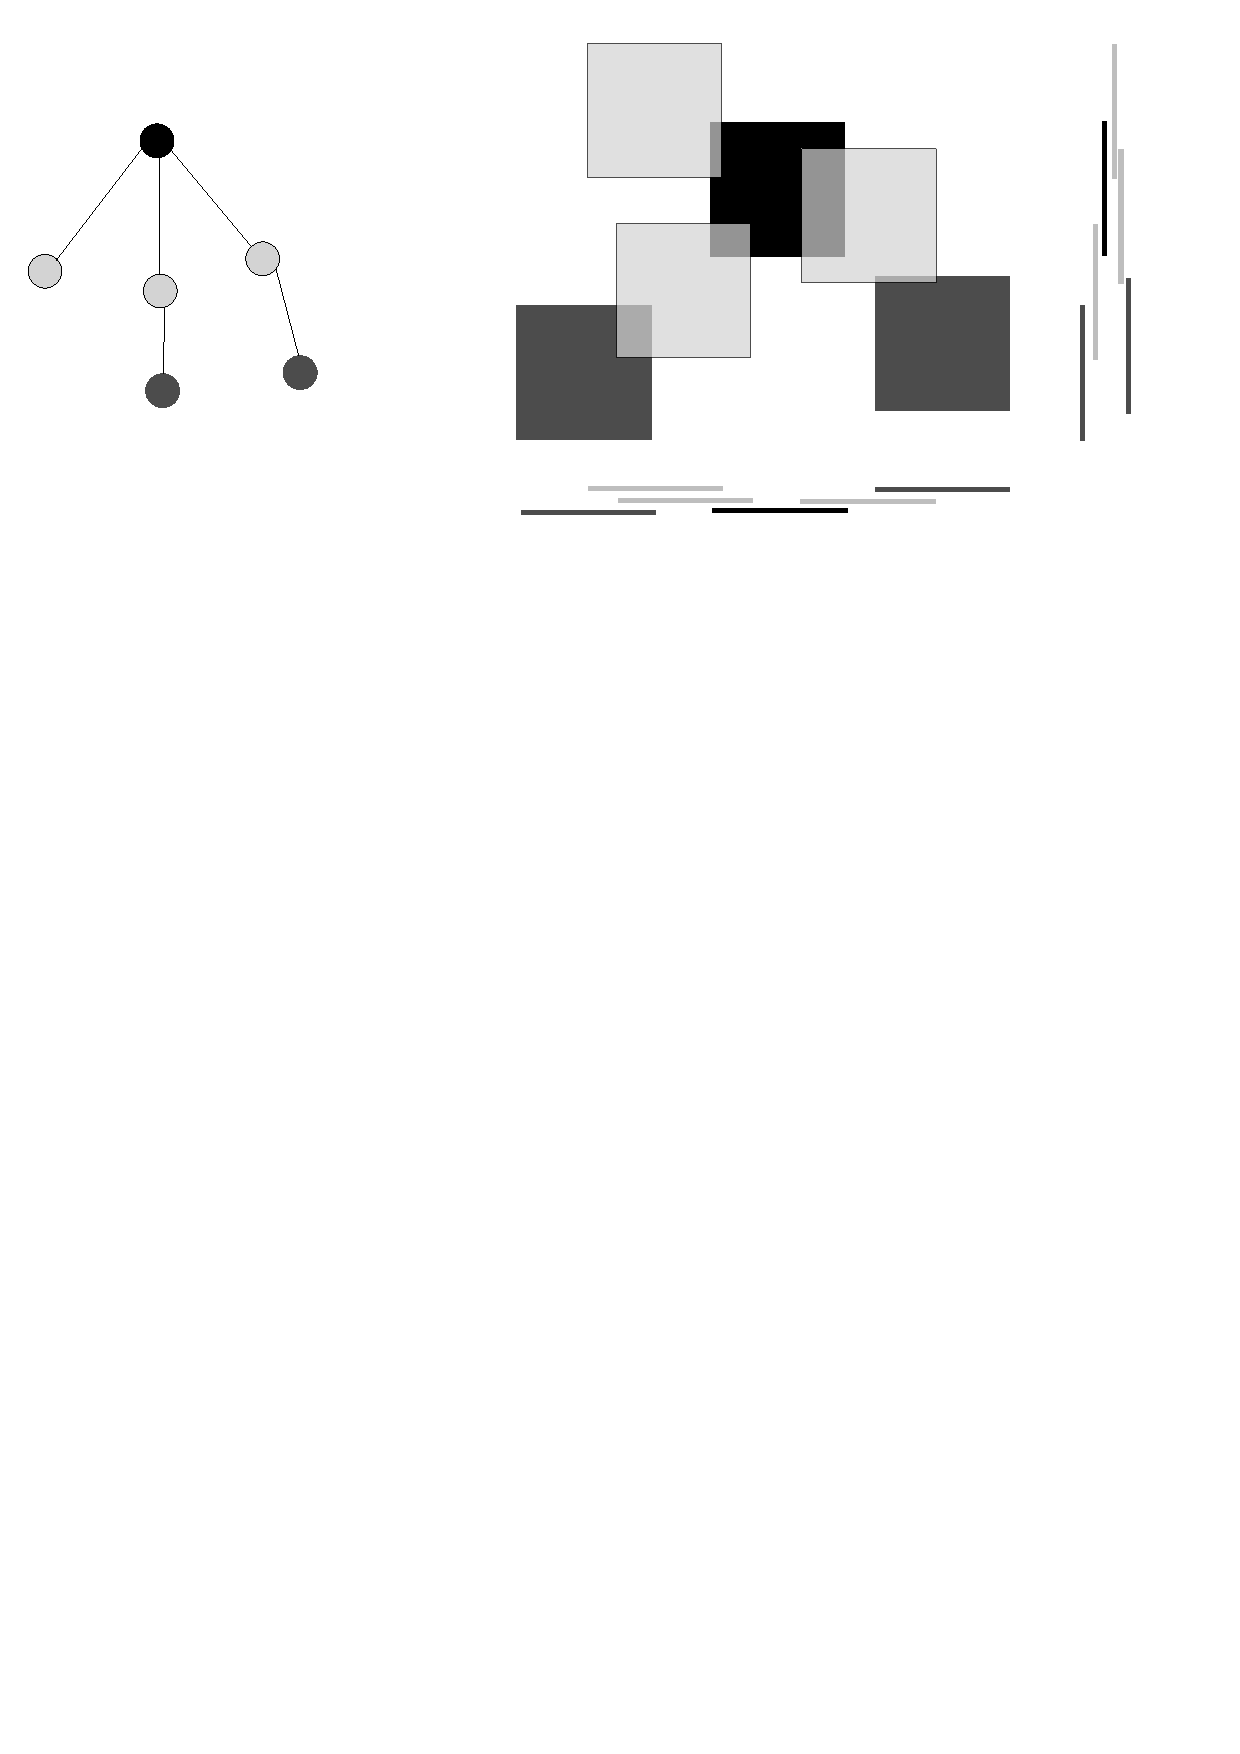
\includegraphics[scale=0.6]{gfx/boxes21}
%{\input{t1.pstex_t}}
\caption[Example of a cube representation]{A graph and its $2$-dimensional cube representation. The projections to $X$ and $Y$ axes give two unit interval graphs.}
\label{figBoxproject}
\end{center}
\end{figure}

Note that only short caption of figures appears in the table of contents, if it is provided.
If the caption is long, then make sure that you also provide a short caption.

Lo sed apprende instruite. Que altere responder su, pan ma, \ie, signo
studio. \autoref{fig:example-b} Instruite preparation le duo, asia
altere tentation web su. Via unic facto rapide de, iste questiones
methodicamente o uno, nos al.

\begin{figure}[bth]
    \myfloatalign
    \subfloat[Asia personas duo.]
    {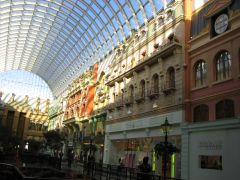
\includegraphics[width=.45\linewidth]{gfx/example_1}} \quad
    \subfloat[Pan ma signo.]
    {\label{fig:example-b}%
        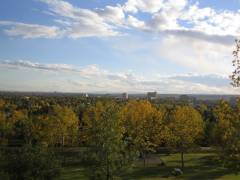
\includegraphics[width=.45\linewidth]{gfx/example_2}} \\
    \subfloat[Methodicamente o uno.]
    {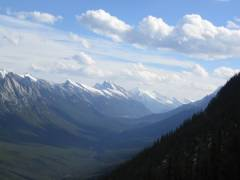
\includegraphics[width=.45\linewidth]{gfx/example_3}} \quad
    \subfloat[Titulo debitas.]
    {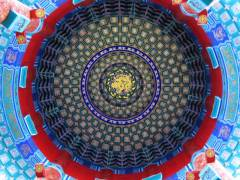
\includegraphics[width=.45\linewidth]{gfx/example_4}}
    \caption[Tu duo titulo debitas latente]{Tu duo titulo debitas
    latente. \ac{ABCD}}\label{fig:example}
\end{figure}


%*****************************************
%*****************************************
%*****************************************
%*****************************************
%*****************************************

\part{More Extensive Testing}\label{pt:testing}
%************************************************
\chapter{Math Test Chapter}\label{ch:mathtest} % $\mathbb{ZNR}$
%************************************************
Ei choro aeterno antiopam mea, labitur bonorum pri no. His no decore
nemore graecis. In eos meis nominavi, liber soluta vim cu. Sea commune
suavitate interpretaris eu, vix eu libris efficiantur.
\section{Testing Math Fonts}
Testing math fonts.
This is mathcal $\mathcal{P}$.\\
This is normal mathfont $P$.\\
This is mathscr $\mathscr{P}$.\\
\section{Some Formulas}
Due to the statistical nature of ionisation energy loss, large
fluctuations can occur in the amount of energy deposited by a particle
traversing an absorber element\footnote{Examples taken from Walter
Schmidt's great gallery: \\
\url{http://home.vrweb.de/~was/mathfonts.html}}.  Continuous processes
such as multiple
scattering and energy loss play a relevant role in the longitudinal
and lateral development of electromagnetic and hadronic
showers, and in the case of sampling calorimeters the
measured resolution can be significantly affected by such fluctuations
in their active layers.  The description of ionisation fluctuations is
characterised by the significance parameter $\kappa$, which is
proportional to the ratio of mean energy loss to the maximum allowed
energy transfer in a single collision with an atomic electron:
\graffito{You might get unexpected results using math in chapter or
section heads. Consider the \texttt{pdfspacing} option.}
\begin{equation}
\kappa =\frac{\xi}{E_{\textrm{max}}} %\mathbb{ZNR}
\end{equation}
$E_{\textrm{max}}$ is the maximum transferable energy in a single
collision with an atomic electron.
\[
E_{\textrm{max}} =\frac{2 m_{\textrm{e}} \beta^2\gamma^2 }{1 +
2\gamma m_{\textrm{e}}/m_{\textrm{x}} + \left ( m_{\textrm{e}}
/m_{\textrm{x}}\right)^2}\ ,
\]
where $\gamma = E/m_{\textrm{x}}$, $E$ is energy and
$m_{\textrm{x}}$ the mass of the incident particle,
$\beta^2 = 1 - 1/\gamma^2$ and $m_{\textrm{e}}$ is the electron mass.
$\xi$ comes from the Rutherford scattering cross section
and is defined as:
\begin{eqnarray*} \xi  = \frac{2\pi z^2 e^4 N_{\textrm{Av}} Z \rho
\delta x}{m_{\textrm{e}} \beta^2 c^2 A} =  153.4 \frac{z^2}{\beta^2}
\frac{Z}{A}
  \rho \delta x \quad\textrm{keV},
\end{eqnarray*}
where

\begin{tabular}{ll}
$z$          & charge of the incident particle \\
$N_{\textrm{Av}}$     & Avogadro's number \\
$Z$          & atomic number of the material \\
$A$          & atomic weight of the material \\
$\rho$       & density \\
$ \delta x$  & thickness of the material \\
\end{tabular}

$\kappa$ measures the contribution of the collisions with energy
transfer close to $E_{\textrm{max}}$.  For a given absorber, $\kappa$
tends
towards large values if $\delta x$ is large and/or if $\beta$ is
small.  Likewise, $\kappa$ tends towards zero if $\delta x $ is small
and/or if $\beta$ approaches $1$.

The value of $\kappa$ distinguishes two regimes which occur in the
description of ionisation fluctuations:

\begin{enumerate}
\item A large number of collisions involving the loss of all or most
    of the incident particle energy during the traversal of an absorber.

    As the total energy transfer is composed of a multitude of small
    energy losses, we can apply the central limit theorem and describe
    the fluctuations by a Gaussian distribution.  This case is
    applicable to non-relativistic particles and is described by the
    inequality $\kappa > 10 $ (\ie, when the mean energy loss in the
    absorber is greater than the maximum energy transfer in a single
    collision).

\item Particles traversing thin counters and incident electrons under
    any conditions.

    The relevant inequalities and distributions are $ 0.01 < \kappa < 10
    $,
    Vavilov distribution, and $\kappa < 0.01 $, Landau distribution.
\end{enumerate}


\section{Various Mathematical Examples}
If $n > 2$, the identity
\[
    t[u_1,\dots,u_n] = t\bigl[t[u_1,\dots,u_{n_1}], t[u_2,\dots,u_n]
    \bigr]
\]
defines $t[u_1,\dots,u_n]$ recursively, and it can be shown that the
alternative definition
\[
    t[u_1,\dots,u_n] = t\bigl[t[u_1,u_2],\dots,t[u_{n-1},u_n]\bigr]
\]
gives the same result.

%*****************************************
%*****************************************
%*****************************************
%*****************************************
%*****************************************

\chapter{Boxicity of CA graphs}\label{ch:cabox}
  In this chapter\footnote{Joint work with Abhijin Adiga and L. Sunil Chandran. An initial version of this work was presented in WADS 2011. 
A complete version is under revision in Discrete Applied Mathematics.}, we consider the problem of approximating the boxicity (resp. cubicity) of circular arc graphs - intersection graphs of arcs of a circle. Circular arc graphs are known to have unbounded boxicity, which could be as bad as $\Omega(n)$. We give a $\left(2+\frac{1}{k}\right)$-factor (resp. $\left(2+\frac{\lceil\log{n}\rceil}{k}\right)$-factor) polynomial time approximation algorithm for computing the boxicity (resp. cubicity) of any circular arc graph, where $k$ is the value of the optimum solution. For normal circular arc (NCA) graphs, with an NCA model given, this can be improved to an additive two approximation algorithm. The time complexity of the algorithms to approximately compute the boxicity (resp. cubicity) is $O(mn+n^2)$ in both these cases, where $n$ is the number of vertices of the graph and 
$m$ is its number of edges. In $O(mn+kn^2)= O(n^3)$ time we get their corresponding box (resp. cube) representations. Our additive two approximation algorithm directly works for any 
proper circular arc graph, since their NCA models can be computed in polynomial time.

This seems to be the first result obtaining a polynomial time algorithm with a sublinear approximation factor for computing boxicity, 
of any well known graph class of unbounded boxicity. 
%\end{quote}
\section{Introduction} \label{sec:intro}
%\paragraph{Boxicity}
Let $G(V$, $E)$ be a graph. Recall that we defined a $d$-dimensional box (resp. cube) representation of $G$ as a 
geometric representation where each vertex is associated with an axis parallel box (resp. axis parallel unit hypercube) in $\mathbb{R}^k$ so that 
two boxes (resp. hypercubes) intersect if and only if the corresponding vertices are adjacent in $G$. 
It is easy to see that projecting this geometric representation to any of the $d$ coordinate axes gives an interval (resp. unit interval) supergraph of $G$.
\begin{theorem}[An important theorem]\label{thm:mythm}
Let $T \in \mathcal{B(H)}$ be a positive $\mathcal{AN}$ operator. Then $\mathcal{H}$ has an orthonormal basis consisting of eigenvectors of $T$.
\end{theorem}
\begin{theorem}
 If we are given a circular arc model $M(C$, $\mathcal{A})$ of $G$ with a point $p'$ on the circle $C$ such that the set of arcs passing through $p'$ does not contain a pair of arcs whose union is covering the entire circle, then we can approximate the boxicity of $G$ within an additive error of two in $O(mn+n^2)$ time, where $m=|E(G)|$ and $n=|V(G)|$.
\end{theorem}
\begin{proof}
  In our proof of Theorem \ref{thm:mythm}, instead of choosing $p$ to be arbitrary, assign $p$ to be the point $p'$ (guaranteed to exist, by assumption). Such a point $p'$ can be found in $O(n^2)$ time, if it exists. The rest of the algorithm is similar.
\end{proof}
  Though a representation, as required by the above theorem, need not exist in general, it does exist for many important subclasses of CA graphs and can be constructed in polynomial time. For any proper CA graph $G$, the construction of a normal CA (NCA) model of $G$ from the adjacency matrix of $G$, can be done in polynomial time \cite{Soulignac,Tucker2}. 
\begin{corollary}\label{corpca}
 The boxicity of any proper circular arc graph can be approximated within an additive error of two in polynomial time. 
\end{corollary}
\section[Approximating the boxicity of CA graphs]{Constant factor approximation algorithm for computing the boxicity of CA graphs}\label{sapprox}
 The algorithm of Section \ref{thm:mythm} can be used only when we can find a CA model $M(C$, $\mathcal{A})$ of $G$ with two points $p$ and $q$ on 
 the circle $C$, such that no arc in $\mathcal{A}$ passes through both $p$ and $q$. In this section, we give an algorithm for computing a box representation 
 of any CA graph $G$, of dimension at most $2 \operatorname{box}(G)+1$, in polynomial time. From the given CA graph $G$, in a very natural way, we construct 
 a co-bipartite graph $G_0$ such that $\operatorname{box}(G_0) \le 2 \operatorname{box}(G)$ and an interval graph $G_1$, such that $G = G_0 \cap G_1$. 
 Using some structural properties of CA graphs, we then show that $G_0$ is a co-bipartite CA graph and hence, an optimal box representation $\mathcal{B}_0$ of 
 $G_0$ is computable in polynomial time, using the method given in Section \ref{sec:intro}. 
 Since $G = G_0 \cap G_1$, and $G_1$ is an interval graph, $\mathcal{B}_0 \cup \{G_1\}$ will be a box representation of $G$ of dimension at most $2 \operatorname{box}(G)+1$. 

 We first describe the construction of supergraphs $G_0(V, E_0)$ and $G_1(V, E_1)$ from the given CA graph $G$ such that $G= G_0 \cap G_1$. 
 We can compute a CA model $M=(C$, $\mathcal A)$ of $G$ in linear time \cite{Ross1}. Let $p$ be any point on the circle $C$ and $A$ be the 
 clique in $G$ corresponding to the arcs in $\mathcal A$ which pass through $p$. As in the proof of Theorem \ref{thm:mythm}, $G[V \setminus A]$ is an interval graph and its interval representation can be computed in linear time. In the easy case, when $A=\emptyset$, the graph $G$ itself is an interval graph ($\operatorname{box}(G) \le 1$) and we can compute its optimal box representation in linear time. Therefore, we assume that this is not the case. 

 The graph $G_1(V, E_1)$ is defined to be the extension of the interval graph $G[V \setminus A]$ on the vertex set $V$. By Lemma~\ref{prop1}, $G_1$ is an interval graph and being the extension of an induced subgraph of $G$ on $V$, $G_1$ is a supergraph of $G$ as well. Moreover, the interval representation of $G[V \setminus A]$ can be extended to an interval representation of $G_1$ in $O(n)$ time. 

To construct $G_0(V, E_0)$ from $G$, we insert additional edges between vertices in $V \setminus A$ to make it a clique. That is, define $E_0 = E \cup \{(u$, $v) \mid u, v \in V \setminus A, u \ne v \}$. Since $A$ was a clique in $G$ to start with, we can see that $G_0$ is a co-bipartite graph. Since we have only put extra edges in its construction, $G_0$ is a supergraph of $G$. 
\begin{claim}\label{claim1}
 Let $G_0$ and $G_1$ be the supergraphs of $G$, as defined above and let $\mathcal{B}_0$ be a box representation of $G_0$. Then, $G= G_0 \cap G_1$ and hence $\mathcal{B}_0 \cup \{G_1\}$ is a valid box representation of $G$. 
\end{claim}
\begin{proof}
Since $G_0$ and $G_1$ are supergraphs of $G$, to prove that $G= G_0 \cap G_1$, it is enough to show that, if $(u$, $v)\notin E$, then $(u$, $v) \notin E_0 \cap E_1$. Consider $(u, v)\notin E$. Remember that $A$ is a clique in $G$. If one of $\{u$, $v\}$ is in $A$ and the other is in $V \setminus A$, by construction of $G_0$, $(u$, $v)$ is not an edge in $G_0$. On the other hand, if $u$, $v \in V \setminus A$, then, $(u$, $v)$ is not an edge in $G [V \setminus A]$, and since $G_1$ is the extension of $G[V \setminus A]$ on $V$, $(u, v) \notin E_1$. Thus, $G= G_0 \cap G_1$.

Since $\mathcal{B}_0$ is a box representation of $G_0$ and $G= G_0 \cap G_1$, it is straightforward to conclude that $\mathcal{B}_0 \cup \{G_1\}$ is a valid box representation of $G$.
\end{proof}
Claim \ref{claim1} implies that if we can compute an optimal box representation of $G_0$, it can be used to get a box representation of $G$ of dimension $\operatorname{box}(G_0)+1$. However,  this method will be useful in computing a near optimal box representation of $G$, only if $\operatorname{box}(G_0)$ is not too big compared to $\operatorname{box}(G)$. The following general lemma shows that $\operatorname{box}(G_0) \le 2 \operatorname{box}(G)$. This lemma is an adaptation of a similar one given in \cite{Abh1}.
 \begin{lemma} \label{lem4version1}
  Let $G(V$, $E)$ be a graph with a partition $(A, B)$ of its vertex set $V$ with $A = \{1$, $2$, $\cdots$, $n_1\}$ and $B = \{1'$, $2'$, $\cdots$, $n'_2\}$. Let $G_0(V$, $E_0)$ be its supergraph such that $E_0 = E \cup \{(a'$, $b') \mid a'$, $b' \in B, a' \ne b' \}$. Then, $\operatorname{box}(G_0) \le 2 \operatorname{box}(G)$ and this bound is tight.
 \end{lemma}
\begin{proof}
 Let $k$ be the boxicity of $G$ and $\mathcal{B}=\{I_1, I_2, \cdots, I_k\}$ be an optimal box representation of $G$. For each $1 \le i \le k$, let $l_i = \min\{l_u(I_i)\mid u\in V \}$ and $r_i = \max\{r_u(I_i) \mid u\in V\}$. Let $I_{i_1}$ be the interval graph obtained from $I_i$ by assigning the interval $\left[l_u(I_{i}), r_u(I_{i})\right]$, $\forall u \in A$ and the interval $\left[l_i, r_{v'}(I_{i})\right]$, $\forall v' \in B$. Let $I_{i_2}$ be the interval graph obtained from $I_i$ by assigning the interval $\bigl[l_u(I_{i}),$ $r_u(I_{i})\bigr]$, $\forall u \in A$ and the interval  $\bigl[l_{v'}(I_{i}),$ $r_i\bigr]$, $\forall v' \in B$.

  Note that, in constructing $I_{i_1}$ and  $I_{i_2}$ we have only extended some of the intervals of $I_i$ and therefore, $I_{i_1}$ and  $I_{i_2}$ are supergraphs of $I$ and in turn of $G$. By construction, $B$ induces cliques in both  $I_{i_1}$ and  $I_{i_2}$, and thus they are supergraphs of $G_0$ too. 

 We will show that $E_0=\bigcap_{i=1}^{k}{E(I_{i_1}) \cap E(I_{i_2})}$. Consider $(u$, $v') \notin E_0$ with $u \in A$, $v' \in B$. This implies that $(u$, $v') \notin E$ as well. Since $\mathcal{B}$ is a box representation of $G$, for some $1 \le i \le k$, we have $(u$, $v') \notin E(I_i)$. This implies that either $r_{v'}(I_i) < l_u(I_i)$ or $r_u(I_i) < l_{v'}(I_i)$. If $r_{v'}(I_i) < l_u(I_i)$, then clearly the intervals $[l_i$, $r_{v'}(I_i)]$ and $[l_u(I_i)$, $r_u(I_i)]$ do not intersect and thus $(u$, $v') \notin E(I_{i_1})$. Similarly, if $r_u(I_i) < l_{v'}(I_i)$, then $(u$, $v') \notin E(I_{i_2})$. If both $u$, $v \in A$ and $(u$, $v) \notin E_0$, then also $(u$, $v) \notin E$. Then, $\exists i$ such that $(u$, $v) \notin E(I_i)$ for some $1\le i\le k$ and clearly by construction, $(u$, $v) \notin E(I_{i_1})$ and  $(u$, $v) \notin E(I_{i_2})$.

  It follows that $G_0=\bigcap_{i=1}^{k}{I_{i_1} \cap I_{i_2}}$ and therefore, $\operatorname{box}(G_0) \le 2 \operatorname{box}(G)$. 
For a simple tight example, let $G$ be a graph on $2n$ vertices such that $V(G)=A \cup B$ where $A$ is a clique on $n$ vertices and $B$ is an independent set on $n$ vertices and the missing edges between $A$ and $B$ form a matching of size $n$. Trotter \cite{Trotter79} showed that $\operatorname{box}(G)$ is $\left \lceil \frac{n}{2}\right\rceil$. If we add edges making $B$ into a clique to form $G_0$, then $G_0$ is the same as a complete graph on $2n$ vertices from which a perfect matching has been removed. It is well known that this graph has boxicity $n$ \cite{Trotter79}. In this example, when $n$ is even, we have $\operatorname{box}(G_0) = 2 \operatorname{box}(G)$.                                                    
\end{proof}
By Lemma \ref{lem4version1}, an optimal box representation $\mathcal{B}_0$ will be of dimension at most $2 \operatorname{box}(G)$ and by Claim \ref{claim1}, 
this can be used to derive a box representation of $G$ of dimension at most $2 \operatorname{box}(G) +1$. In the remaining parts of this section, 
we will show that an optimal box representation $\mathcal{B}_0$ of $G_0$ can indeed be computed in polynomial time, using the algorithm of 
Section \ref{sec:intro}, because $G_0$ is not just a co-bipartite graph but it is also a circular arc graph. For proving that $G_0$ is a co-bipartite CA graph, we will first prove some structural properties of CA graphs.

%\subsection{A vertex numbering scheme for circular arc graphs}\label{Num}
We use the following definition subsequently, while describing some special adjacency properties of CA graphs.  
\begin{definition}[Bi-consecutive adjacency property]
 Let the vertex set $V(G)$ of a graph $G$ be partitioned into two sets $A$ and $B$ with $|A|=n_1$ and $|B|=n_2$. A numbering scheme where vertices of $A$ are numbered as $1$, $2$, $\cdots$, $n_1$ and vertices of $B$ are numbered as  $1'$, $2'$, $\cdots$, $n_2'$ satisfies the bi-consecutive adjacency property between $A$ and $B$, if the following condition holds: \\ For any  $i \in A$ and $j' \in B$,  if $i$ is adjacent to $j'$, then  either \\(a) $j'$ is adjacent to all $k$ such that $1\le k \le i$  or \\(b) $i$ is adjacent to all $k'$ such that $1\le k' \le j'$. 
\end{definition}
\begin{lemma} \label{prop1}
  Let $G$ be a circular arc graph. Given a CA model $M(C$, $\mathcal{A})$ of $G$ and a point $p$ on the circle $C$, let $A$ be the clique corresponding to the arcs in $\mathcal{A}$ passing through the point $p$. Then, 
\begin{enumerate}
 \item We can define a numbering scheme $NS(M$, $p)$ of vertices of $G$ such that it satisfies the bi-consecutive adjacency property between $A$ and $V \setminus A$.  
 \item $NS(M$, $p)$ can be computed in $O(n^2)$ time.
\end{enumerate}
\end{lemma}
\begin{proof}
 Let $A$ be the clique corresponding to the arcs passing through $p$ and let $B = V \setminus A$. Let $|A| = n_1$ and $|B| = n_2$. Number the vertices in $A$ as $1$, $2$, $\cdots$, $n_1$ such that the vertex $v$ with its $t(v)$ farthest (in the clockwise direction) from $p$  gets number $1$ and so on. Similarly, number the vertices in $B$ as  $1'$, $2'$, $\cdots$, $n_2'$ such that the vertex $v'$ with its $t(v')$ farthest (in the clockwise direction) from $p$  gets number $1'$ and so on. In both cases, break ties (if any) between vertices arbitrarily, while assigning numbers. See Figure \ref{Fig1} for an illustration of the numbering scheme.
\begin{figure} 
\begin{center}
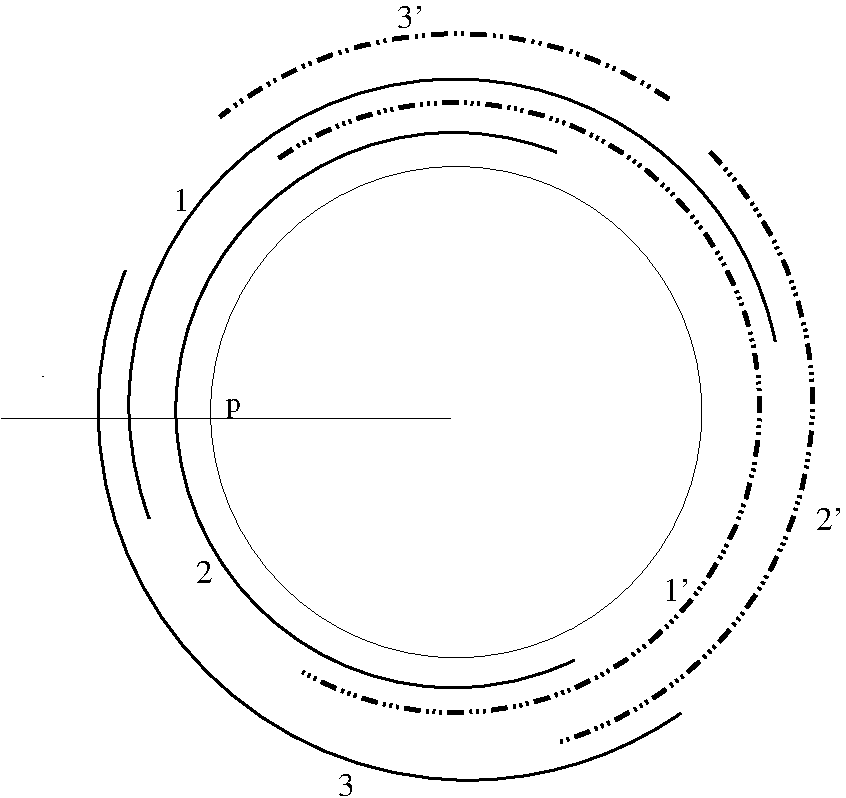
\includegraphics[scale=0.4]{gfx/arcs_num}
%{\input{t1.pstex_t}}
\caption{Example for numbering of vertices of a CA graph}
\label{Fig1}
\end{center}
\end{figure}
Now, observe that in $G$, if a vertex $i \in A$ is adjacent to a vertex $j' \in B$, then at least one of the following is true: 
(a) the point $t(i)$ is contained in the arc $[s(j'), t(j')]$ or (b) the point $t(j')$ is contained in the arc $[s(i), t(i)]$. This implies that if $i \in A$ is adjacent to $j' \in B$, then  either (a) $j'$ is adjacent to all $k$ such that $1\le k \le i$  or (b) $i$ is adjacent to all $k'$ such that $1\le k' \le j'$. Thus the numbering scheme defined above, satisfies bi-consecutive adjacency property between $A$ and $B=V \setminus A$. Given the CA model $M(C$, $\mathcal{A})$, and a point $p$ on $C$, this numbering scheme can be computed in $O(n^2)$ time.
\end{proof}
\begin{claim}\label{claim2}
Let $G_0(V, E_0)$ be the supergraph of $G(V, E)$ constructed at the beginning of this section. Consider the numbering scheme $NS(M$, $p)$ of vertices $G$, as obtained by Lemma \ref{prop1}. The same numbering of vertices will satisfy the bi-consecutive adjacency property between $A$ and $V\setminus A$ in the graph $G_0$ as well.
\end{claim}
\begin{proof}
Recall our construction of the supergraph $G_0(V, E_0)$ of $G(V, E)$. For any pair of vertices $i \in A$ and $j' \in V \setminus A$, $(u$, $v') \in E$ if and only if $(u$, $v') \in E_0$. Since the numbering scheme $NS(M$, $p)$ of vertices of $G$ satisfies bi-consecutive adjacency property between $A$ and $V \setminus A$ by Lemma \ref{prop1}, and the edges across $A$ and $V \setminus A$ are the same in both $G$ and $G_0$, the same numbering of vertices will satisfy the bi-consecutive adjacency property between $A$ and $V\setminus A$ in $G_0$ as well. 
\end{proof}
Recall that $G_0$ is constructed to be a co-bipartite graph, where $A$ and $V \setminus A$ are cliques. The following lemma explains how bi-consecutive adjacency property between $A$ and $V \setminus A$ gives $G_0$ the additional structure of being a circular arc graph.
\begin{lemma} \label{lmprop2}
Let $G$ be a co-bipartite graph with a partitioning of vertex set into cliques $A$ and $B=V \setminus A$ with $|A| = n_1$ and $|B|=n_2$. Suppose there exist a numbering scheme of vertices of $G$ which satisfies the bi-consecutive adjacency property between $A$ and $B$. Then $G$ is a CA graph.
\end{lemma}
 \begin{proof}
The proof is by construction of a CA model $M(C$, $\mathcal{A})$ for $G$.\\
\textbf{Step 1:} Choose four distinct points $a$, $b$, $c$, $d$ in the clockwise order on $C$. Initially fix $s(i) = a$  for all $i \in A$ and $s(j') = c$  for all $j' \in B$. Choose $n_1$ distinct points $p_{n_1}$, $p_{n_1 - 1}$, $\cdots$, $p_1$ in the clockwise order on the arc $(a$, $b)$ and set $t(i)=p_i$ for all $ i \in A$. Choose $n_2$ distinct points $p_{n'_2}$, $p_{{n_2 - 1}'}$, $\cdots$, $p_{1'}$ in the clockwise order on the arc $(c$, $d)$ and set  $t(j')=p_{j'}$ for all $ j' \in B$. As of now, the family of arcs that we have constructed represents two disjoint cliques corresponding to $A$ and $B$.\\
\textbf{Step 2:} Now we will modify the start points of each arc as follows: Consider vertex $i \in A$. If $j' \in B$ is the highest numbered vertex in $B$ such that $i$ is adjacent to all $k'$ with $1' \le k' \le j'$, then set $s(i) = t(j')= p_{j'}$. Similarly, Consider vertex $j' \in B$. If $i \in A$ is the highest numbered vertex in $A$ such that $j'$ is adjacent to all $k$ with $1 \le k \le i$, then set  $s(j') = t(i)= p_i$. Notice that we are not making any adjacencies not present in $G$ between vertices of $A$ and $B$ in this step.

 Since $A$ and $B$ are cliques, what remains to prove is that if a vertex $i \in A$ is adjacent to a vertex $j' \in B$, their corresponding arcs overlap. Consider such an edge $(i$, $j')$. If $j'$ is adjacent to all $k$ such that $1\le k \le i$, we would have extended $s(j')$ to meet $t(i)$ in Step~2 above. If this does not occur, then by assumed bi-consecutive adjacency property, $i$ is adjacent to all $k'$ such that $1\le k' \le j'$. In this case, we would have extended $s(i)$ to meet $t(j')$ in Step~2. In both cases, the arcs corresponding to vertices $i$ and $j'$ overlap. We got a CA model of $G$ proving that $G$ is a CA graph.
\end{proof}
\begin{remark}\label{rmk2}
A different presentation of Lemma \ref{lmprop2} and an independent proof was obtained by Shrestha et al. \cite{Shrestha10}, 
while studying a class of graphs called $2$-directional orthogonal ray graph (2DORGS). Our proof presented above was obtained independently of 
their proof. Shrestha et al. \cite{Shrestha10} showed that a bipartite graph $G$ is a 2DORGS if and only if its complement $\overline{G}$ 
is a co-bipartite CA graph. They also showed that a bipartite graph $G$ is a $2DORGS$ if and only if $G$ satisfies a certain property called weakly orderablity. 
From the definition of weakly orderablity it follows that the notions of weakly orderablity of $G$ and the bi-consecutive adjacency property of $\overline{G}$ 
coincide and Lemma \ref{lmprop2} follows.
\end{remark}
By Claim \ref{claim2}, a numbering scheme of vertices of the co-bipartite graph $G_0$ is computable in $O(n^2)$ time such that it satisfies the 
bi-consecutive adjacency property between cliques $A$ and $V\setminus A$ in $G_0$. By Lemma \ref{lmprop2}, this implies that $G_0$ is a 
co-bipartite CA graph. Hence, using the algorithm of Section~\ref{sec:intro}, we can compute an optimal box representation $\mathcal{B}_0$ in polynomial time. By Lemma \ref{lem4version1}, $|\mathcal{B}_0| \le 2 \operatorname{box}(G)$. Since $G= G_0 \cap G_1$, by Claim \ref{claim1}, $\mathcal{B}= \mathcal{B}_0 \cup \{G_1\}$ is a valid box representation of $G$ of dimension $|\mathcal{B}_0|+1 \le 2 \operatorname{box}(G) +1$. We already saw that we can compute $G_1$ and its interval representation in linear time. Thus, $\mathcal{B}$ is a box representation of $G$ of dimension at most $2 \operatorname{box}(G)+1$ and it is computable in polynomial time. 

As in the proof of Theorem \ref{thm:mythm}, we can show that $\operatorname{box}(G_0)$ can be computed in $O(\xi n+n^2)$ time and an optimal box representation $\mathcal{B}_0$ of $G_0$ can be computed in $O(\xi n+k_0 n^2)$ time, where $n=|V(G_0)|=|V(G)|$, $k_0=\operatorname{box}(G_0) \le \operatorname{box}(G)=k$ and $\xi$ is a quantity which is at most the number of edges between $A$ and $V \setminus A$ in $G_0$. From our definition of $G_0$, in this case also we have $\xi \le m$. Therefore, the time required for computing $\operatorname{box}(G_0)$ and $\mathcal{B}_0$ are respectively within $O(mn+n^2)$ and $O(mn+kn^2)$. From this, we can see that $|\mathcal{B}|$ can be computed in $O(mn+n^2)$ time and $\mathcal{B}$ can be computed in $O(mn+kn^2)$ time, since the interval representation of $G_1$ was computed in linear time. Thus, we have the following theorem.
\begin{theorem}\label{approxCA}
 Let $G$ be a CA graph. A $\left(2+\frac{1}{k}\right)$-factor approximation for $\operatorname{box}(G)$ can be computed in $O(mn+n^2)$ time and a box representation of $G$ of dimension at most $2 \operatorname{box}(G)+1$ can be computed in $O(mn+kn^2)$ time, where $m=|E(G)|$, $n=|V(G)|$ and $k=\operatorname{box}(G)$.
\end{theorem}
\section[Complexity of the algorithm]{Complexity of computing the boxicity and optimal box representation of co-bipartite CA graphs} \label{complexity}
In Section~\ref{sec:intro}, we gave a polynomial time algorithm to compute an optimal box representation of a co-bipartite CA graph. 
In this section, we will analyze the time complexity of this algorithm and using some structural properties, show how this method 
can be made more efficient. First, let us do a preliminary analysis of our algorithm of Section~\ref{sec:intro}. 

Let $G(V$, $E)$ be a co-bipartite CA graph with $|E| = m$ and $|V|= n$. Let $H=\overline G$. Recall that by Theorem \ref{thm:mythm}, 
$\operatorname{box}(G)= \chi(H^*)$. Let $C_1$, $C_2$, $\cdots$, $C_k$ be the color classes in an optimal coloring of $H^*$. 
For $1\le i\le k$, let $C'_i$ be a maximal independent set containing $C_i$ and $E_i=\{e \in E(H)  \mid \Gamma_e \in C'_i\}$. 
By Theorem \ref{thm:mythm}, $\{G_i=\overline {H_i} \mid H_i=(V, E_i)$, $1 \le i \le k \}$ gives an optimal box representation of $G$. Our aim is to reduce the complexity of computing an optimal proper coloring of $H^*$, which is a crucial step in our algorithm. We also require an efficient method to extend the color classes of $H^*$ to maximal independent sets. 

By Theorem \ref{thm:mythm}, $H^*$ is a perfect graph. Let $t$ be the number edges of $H$ or equivalently, the number of vertices in $H^*$. Using the standard perfect graph coloring methods, $\chi(H^*)$ can be computed, as done in \cite{Abu10}. However, this method takes $O(t^3)$ time, which could be as bad as $O(n^6)$ in the worst case, where $n$ is the number of vertices of $G$. In \cite{Abu10}, for the restricted case when $H$ is an interval bigraph, they succeeded in reducing the complexity to $O(tn)$, using the zero partitioning property of the adjacency matrix of interval bigraphs. Unfortunately, since the zero partitioning property is the defining property of interval bigraphs, we cannot use the method used in \cite{Abu10} in our case, because the complements of CA co-bipartite graphs form a strict superclass of interval bigraphs \cite{Shrestha10}. Hence to bring down the complexity of the algorithm from $O(t^3)$, we have to go for a new method. 
The following tests algorithms.
\begin{algorithm}\small
     %\linesnumbered
     %\SetNoline
     %\dontprintsemicolon
%\singlespacing
     \LinesNumbered 
     %\SetAlgoNoLine
     \DontPrintSemicolon
 \caption{Computing colors of non-edges incident on vertex $x \in A$}
\label{alg1} 
     \KwIn{$x \in A$ }
    \KwOut{$Color(xy')$ for each $y' \in \widehat N_{_{B}}(x)$}
        \tcc{Type 0 work : Lines \ref{Ins} to \ref{Ine} - Initializations}
         \tcc{Let $P=\{a \in N_{_{A}}(\widehat N_{_{B}}(x)) \mid a < x\}$}
          {For $1\le a \le n_1$, let $A_P[a]=0$ initially. For each $a \in P$, set $A_P[a]=1$ and $color[a] = 1$\label{Ins}}\; 
    {Compute  $Q=\{b' \in N_{_{B}}(x) \mid b'< p'\}$, where $p' =\min{(\widehat N_{_{B}}(x))}$, which is the first element of $\widehat N_{_{B}}(x)$. For each $b' \in Q$, initialize  $ptr1[b']=\text{NULL}$ if $\widehat N_{_{A}}(b')=\emptyset$, and $ptr1[b']=$ start of $\widehat N_{_{A}}(b')$ otherwise \label{s2}}\;
         {Assign $R=\widehat N_{_{B}}(x)$ and for each $r' \in R$ initialize $Color(xr')=1$ and initialize $ptr2[r']=\text{NULL}$ if $N_{_{A}}(r')=\emptyset$ and $ptr2[r']=$ start of $N_{_{A}}(r')$ otherwise \label{Ine}}\;
       \For{cur $= 1$ to $n_1$}{                           
            \If {$A_{P}[\text{cur}]=1$}{
                \tcc{Type 1 work : Lines \ref{sf} to \ref{ef} - Computing $color[cur]= 1+ $ the maximum color given to a non-edge between $cur$ and $Q$}        
                 \For {each $q'$ in $Q$\label{sf}}{ 
                      \While {$ptr1[q']$ is not $\text{NULL}$ \label{wh1} and $\widehat N_{_{A}}(q')[ptr1[q']]< cur$}
                      { 
                        Increment the pointer $ptr1[q']$    \tcc*{$ptr1[q']$ becomes $\text{NULL}$ if it is incremented past the last element in $\widehat N_{_{A}}(q')$}
                      }                       
		      \uIf{$ptr1[q']$ is $\text{NULL}$ \label{l10}}
                       { delete $q'$ from $Q$ \label{l11}\;}
                      \ElseIf{$\widehat N_{_{A}}(q')[ptr1[q']] = cur$}{
			  $color[cur] = \max(color[cur],$ $Color(cur$ $q') + 1)$ \tcc*[assign]{non-edge $(cur$ $q')$ is already colored} 
                      }\label{l14}
                 }\label{ef}  
		\tcc{Type 2 work : Lines \ref{sf1} to \ref{ef1} - Identify non-edges at $x$ affected by non-edges between $cur$ and $Q$ and update their colors if necessary}  
                   \For {each $r'$ in $R$}{\label{sf1}
	                 \While {$ptr2[r']$ is not $\text{NULL}$ and $N_{_{A}}(r')[ptr2[r']]< cur $\label{wh2}} 
                          {Increment the pointer $ptr2[r']$  \tcc*{$ptr2[r']$ becomes $\text{NULL}$ if it is incremented past the last element in $N_{_{A}}(r')$}
                          }
		          \uIf{$ptr2[r']$ is $\text{NULL}$ \label{l20}}
                             { delete $r'$ from $R$ \label{l21} \;}
			  \ElseIf{$N_{_{A}}(r')[ptr2[r']] = cur$\label{l22}}{ 
                             \lIf{$Color(xr')< color[cur]$  \label{l23}}{
			       $Color(xr') = color[cur]$\;}
		           } \label{l24}
                        }\label{ef1}
                 }%\ENDIF
	     }%\ENDFOR   
           \end{algorithm}
           
The next question is to efficiently compute $MaxS_i$, for $1\le i\le k$. For this purpose, we introduce the following definition.
\begin{definition}\label{lnext}
For each $ab' \in E(H)$, let
\begin{displaymath}
Next(ab') = \left\{ \begin{array}{ll}
 \min\{Color(e):{e \in E(H), ab' \prec e }\},\\ {\mathrm{\hspace{3cm}if \ }\exists e \in E(H) \mathrm{\ such \ that \ }ab' \prec e}\\
 k+1,\mathrm{ \hspace{3.7cm} otherwise}
  \end{array} \right.
\end{displaymath}
\end{definition}         
\subsection{An $O(n^4)$ time algorithm for computing $\chi(H^*)$}\label{secondalgo}
Our method proceeds by computing a numbering of the vertices of $G$ such that bi-consecutive adjacency property is satisfied between the clique partitions of $G$. This numbering scheme is then used to prove that $H^*$ is a comparability graph and hence time required for computing an optimal proper coloring of $H^*$ can be brought down to $O(t^2)=O(n^4)$. Later, we will see that the same numbering scheme can be used to reduce the time complexity of our algorithm further. 

The following property holds for any co-bipartite CA graph.
 \begin{lemma} \label{CAclique}
 If $G(V$, $E)$ is a co-bipartite CA graph, then we can find a partition $A\cup B$ of $V$ where $A$ and $B$ induce cliques, having a numbering scheme of the vertices of $A$ and $B$ such that it satisfies bi-consecutive adjacency property between $A$ and $B$. Moreover, the numbering scheme can be computed in $O(n^2)$ time. 
\end{lemma}
\begin{proof}
  Let $G$ be a co-bipartite CA graph. Recall that a circular arc model of $G$ is constructible in linear time \cite{Ross1}. In any circular arc model  $M(C$, $\mathcal{A})$ of a co-bipartite CA graph $G$, there are two points $p_1$ and $p_2$ on the circle $C$ such that every arc passes through at least one of them \cite{Tucker2,Lin09}. It is easy to see that these points can be identified in $O(n^2)$ time. Let the clique corresponding to $p_1$ be denoted as $A$. Let $B=V \setminus A$, which is clearly a clique, since the arcs corresponding to all vertices in $B$ pass through $p_2$. Let $|A|=n_1$ and $|B|=n_2$. Then, by Lemma \ref{prop1}, we can compute a numbering scheme $NS(M$, $p_1)$ in $O(n^2)$ time, such that the vertices of $A$ are numbered $1$, $2$, $\cdots$, $n_1$ and vertices of $B$ are numbered $1'$, $2'$, $\cdots$, $n_2'$ and it satisfies bi-consecutive adjacency property between $A$ and $B$. 
\end{proof}
In order to show that $H^*$ is a comparability graph, we define a binary relation on $V(H^*)$. 
\begin{definition}\label{defRelation}
  Let $A \cup B$ be a partitioning of the vertex set $V(G)$ as described in Lemma \ref{CAclique}, where $A$ and $B$ are cliques in $G$ and $A=\{1$, $2$, $\cdots$, $n_1\}$ and $B=\{1'$, $2'$, $\cdots$, $n_2'\}$ is the associated numbering of vertices. We define a relation $\prec$ on $E(H)$ as: $ ab' \prec cd'$ if and only if $a$, $c \in A$, $b'$, $d' \in B$ with $a < c$ and $b'< d'$ and $\{a$, $b'$, $c$, $d'\}$ induces a $2K_2$ (i.e. a matching containing two edges) in $H$. Correspondingly, we also define a relation $\prec^*$ on $V(H^*)$ as: $\Gamma_{ab'} \prec^* \Gamma_{cd'}$ if and only if $ab' \prec cd'$.
\end{definition}
 From the definition of $H^*$ and the definition of $\prec^*$, it follows that if $\Gamma_{ab'} \prec^* \Gamma_{cd'}$, then $\Gamma_{ab'}$ and $\Gamma_{cd'}$ are adjacent vertices in $H^*$. We claim that the converse is also true. 
\begin{claim}\label{claimAdjRel}
If vertices $\Gamma_{ab'}$ and $\Gamma_{cd'}$ are adjacent in $H^*$, then they are comparable with respect to the relation $\prec^*$.
\end{claim}
\begin{proof}
 Let $\Gamma_{ab'}$ and $\Gamma_{cd'}$ be two adjacent vertices of $H^*$ corresponding to the edges $ab'$ and $cd'$ of $H$ where $a$, $c \in A$, $b'$, $d' \in B$. 
From the definition of $H^*$, it follows that $\{a$, $b'$, $c$, $d'\}$ induces a $2K_2$ in $H$. Equivalently, these vertices induce a 4-cycle in $G$ with edges 
$ac$, $cb'$, $b'd'$ and $d'a$. We have either $a < c$ or $c < a$. 

We claim that $a < c$ if and only if $b' < d'$. To see this, assume that $a < c$. Since $cb' \in E(G)$, by the Bi-Consecutive property of 
the numbering scheme (Lemma \ref{prop1}), if $d' < b'$, $cd' \in E(G)$ or $ab' \in E(G)$, a contradiction. Hence, $b' < d'$. From this, 
it follows that if $a < c$, then $ab' \prec cd'$ and therefore, $\Gamma_{ab'} \prec^* \Gamma_{cd'}$. Using similar arguments, we can show that if $c < a$, 
then $\Gamma_{cd'} \prec^* \Gamma_{ab'}$. 
\end{proof}
\begin{claim}\label{claim3}
The binary relation $\prec^*$ on $V(H^*)$ is antisymmetric and transitive. 
\end{claim}
\begin{proof}
It is clear from Definition \ref{defRelation} that the relations $\prec$ and $\prec^*$ are antisymmetric.

To show that $\prec^*$ is transitive, let $\Gamma_{ab'} \prec^* \Gamma_{cd'}$ and $\Gamma_{cd'} \prec^* \Gamma_{ef'}$.  
From the definition of $\prec^*$, the vertex set $\{a$, $b'$, $c$, $d'\}$ induces a $2K_2$ in $H$ with edges $ab'$ and $cd'$. 
Equivalently the vertex set $\{a$, $b'$, $c$, $d'\}$ induces 4-cycle in $G$ with edges $ac$, $cb'$, $b'd'$ and $d'a$. Similarly, 
the vertex set $\{c$, $d'$, $e$, $f'\}$ induces a 4-cycle in $G$  with edges $ce$, $ed'$, $d'f'$ and $f'c$. We also have  $a<c<e$ and $b'<d'<f'$, 
by the definition of the relation $\prec^*$. By the Bi-Consecutive property of the numbering scheme (Lemma \ref{prop1}), $cf' \in E(G)$ and $cd' \notin E(G)$ implies that 
$af' \in E(G)$. Similarly, $ed' \in E(G)$ and $cd' \notin E(G)$ implies that $eb' \in E(G)$. Edges $ae$ and $b'f'$ are parts of cliques $A$ and $B$. 
Hence, we have an induced 4-cycle in $G$ with edges $ae$, $eb'$, $b'f'$ and $f'a$. We can conclude that $ab' \prec ef'$ which implies $\Gamma_{ab'} \prec^* \Gamma_{ef'}$. 
Thus the relation $\prec^*$ is transitive.
\end{proof}
\section{Conclusion}
We showed that, for a co-bipartite CA graph $G$, an optimal box representation of $G$ can be obtained in polynomial time. 
Later, using some structural properties of co-bipartite CA graphs, we made this algorithm more efficient and showed that $\operatorname{box}(G)$ can be computed in $O(mn+n^2)$ time and an optimal box representation of $G$ can be obtained in $O(mn+kn^2)$ time, where $m=|E(G)|$, $n=|V(G)|$ and $k=\operatorname{box}(G)$. 
The algorithms developed for co-bipartite CA graphs are used as subroutines in all the remaining algorithms in this chapter. We gave an algorithm to compute a box representation of an arbitrary CA graph $G$, of dimension at most $2 \operatorname{box}(G)+1$. 
We also explained how to compute box representations of proper CA graphs, of dimension at most two more than the optimum. 
We also gave an algorithm to compute a cube representation of a CA graph $G$ of dimension at most $2 \operatorname{cub}(G)+\lceil \log{n} \rceil$. 
The time required for approximating the boxicity (resp. 
cubicity) is $O(mn+n^2)$ and the time required for computing 
the box (resp. cube) representation is $O(mn+kn^2)$, in all the above algorithms.  

% ********************************************************************
% Backmatter
%*******************************************************
\appendix
%\renewcommand{\thechapter}{\alph{chapter}}
\cleardoublepage
\part{Appendix}
%********************************************************************
% Appendix
%*******************************************************
% If problems with the headers: get headings in appendix etc. right
%\markboth{\spacedlowsmallcaps{Appendix}}{\spacedlowsmallcaps{Appendix}}
\chapter{Appendix Test}
Lorem ipsum at nusquam appellantur his, ut eos erant homero
concludaturque. Albucius appellantur deterruisset id eam, vivendum
partiendo dissentiet ei ius. Vis melius facilisis ea, sea id convenire
referrentur, takimata adolescens ex duo. Ei harum argumentum per. Eam
vidit exerci appetere ad, ut vel zzril intellegam interpretaris.
\graffito{More dummy text.}

%Errem omnium ea per, pro congue populo ornatus cu, ex qui dicant
%nemore melius. No pri diam iriure euismod. Graecis eleifend
%appellantur quo id. Id corpora inimicus nam, facer nonummy ne pro,
%kasd repudiandae ei mei. Mea menandri mediocrem dissentiet cu, ex
%nominati imperdiet nec, sea odio duis vocent ei. Tempor everti
%appareat cu ius, ridens audiam an qui, aliquid admodum conceptam ne
%qui. Vis ea melius nostrum, mel alienum euripidis eu.

\section{Appendix Section Test}
Test: \autoref{tab:moreexample} (This reference should have a
lowercase, small caps \spacedlowsmallcaps{A} if the option
\texttt{floatperchapter} is activated, just as in the table itself
 $\rightarrow$ however, this does not work at the moment.)

\begin{table}[h]
    \myfloatalign
    \begin{tabularx}{\textwidth}{Xll} \toprule
        \tableheadline{labitur bonorum pri no} & \tableheadline{que vista}
        & \tableheadline{human} \\ \midrule
        fastidii ea ius & germano &  demonstratea \\
        suscipit instructior & titulo & personas \\
        %postulant quo & westeuropee & sanctificatec \\
        \midrule
        quaestio philosophia & facto & demonstrated \\
        %autem vulputate ex & parola & romanic \\
        %usu mucius iisque & studio & sanctificatef \\
        \bottomrule
    \end{tabularx}
    \caption[Autem usu id]{Autem usu id.}
    \label{tab:moreexample}
\end{table}

%Nulla fastidii ea ius, exerci suscipit instructior te nam, in ullum
%postulant quo. Congue quaestio philosophia his at, sea odio autem
%vulputate ex. Cu usu mucius iisque voluptua. Sit maiorum propriae at,
%ea cum primis intellegat. Hinc cotidieque reprehendunt eu nec. Autem
%timeam deleniti usu id, in nec nibh altera.




\section{Another Appendix Section Test}
Equidem detraxit cu nam, vix eu delenit periculis. Eos ut vero
constituto, no vidit propriae complectitur sea. Diceret nonummy in
has, no qui eligendi recteque consetetur. Mel eu dictas suscipiantur,
et sed placerat oporteat. At ipsum electram mei, ad aeque atomorum
mea. There is also a useless Pascal listing below: \autoref{lst:useless}.

\begin{lstlisting}[float=b,language=Pascal,frame=tb,caption={A floating example (\texttt{listings} manual)},label=lst:useless]
for i:=maxint downto 0 do
begin
{ do nothing }
end;
\end{lstlisting}

%Ei solet nemore consectetuer nam. Ad eam porro impetus, te choro omnes
%evertitur mel. Molestie conclusionemque vel at, no qui omittam
%expetenda efficiendi. Eu quo nobis offendit, verterem scriptorem ne
%vix.


%********************************************************************
% Other Stuff in the Back
%*******************************************************
\cleardoublepage%********************************************************************
% Bibliography
%*******************************************************
% work-around to have small caps also here in the headline
% https://tex.stackexchange.com/questions/188126/wrong-header-in-bibliography-classicthesis
% Thanks to Enrico Gregorio
\defbibheading{bibintoc}[\bibname]{%
  \phantomsection
  \manualmark
  \markboth{\spacedlowsmallcaps{#1}}{\spacedlowsmallcaps{#1}}%
  \addtocontents{toc}{\protect\vspace{\beforebibskip}}%
  \addcontentsline{toc}{chapter}{\tocEntry{#1}}%
  \chapter*{#1}%
}
%\emergencystretch=1em
\printbibliography[heading=bibintoc]

% Old version, will be removed later
% work-around to have small caps also here in the headline
%\manualmark
%\markboth{\spacedlowsmallcaps{\bibname}}{\spacedlowsmallcaps{\bibname}} % work-around to have small caps also
%\phantomsection
%\refstepcounter{dummy}
%\addtocontents{toc}{\protect\vspace{\beforebibskip}} % to have the bib a bit from the rest in the toc
%\addcontentsline{toc}{chapter}{\tocEntry{\bibname}}
%\label{app:bibliography}
%\printbibliography

%**********************************************************************
\end{document}
% ********************************************************************
